% !TeX encoding = UTF-8

% 载入 SJTUThesis 模版
\documentclass[type=master, openany]{sjtuthesis}
% 选项
%   type=[doctor|master|bachelor],     % 可选(默认:master),论文类型
%   zihao=[-4|5],                      % 可选(默认:-4),正文字号大小
%   lang=[zh|en|de|ja],                % 可选(默认:zh),论文的主要语言
%   review,                            % 可选(默认:关闭),盲审模式
%   [twoside|oneside],                 % 可选(默认:twoside),双页或单页边距模式
%   [openright|openany],               % 可选(默认:openright),奇数页或任意页开始新章
%   math-style=[ISO|TeX],              % 可选 (默认:ISO),数学符号样式

% 论文基本配置,加载宏包等全局配置
% !TEX root = ./main.tex

\sjtusetup{
  %
  %******************************
  % 注意:
  %   1. 配置里面不要出现空行
  %   2. 不需要的配置信息可以删除
  %******************************
  %
  % 信息录入
  %
  info = {%
    %
    % 标题
    %
    zh / title           = {基于静态单赋值中间语言的函数式编译器\\ 验证方法},
    en / title           = {Verification of Functional Compilers Based on Static Single Assignment Intermediate Representation},
    %
    % 标题页标题
    %   可使用“\\”命令手动控制换行
    % 
    % zh / display-title   = {上海交通大学学位论文\\ \LaTeX{} 模板示例文档},
    % en / display-title   = {A Sample Document \\ for \LaTeX-based SJTU Thesis Template},
    %
    % 关键词
    %
    zh / keywords        = {编译器验证, 形式化方法, 静态单赋值, 函数式编译器},
    en / keywords        = {Compiler Verification, Formal Methods, Static Single Assignment, Functional Compilers},
    %
    % 姓名
    %
    zh / author          = {刘思雨},
    en / author          = {Siyu Liu},
    %
    % 指导教师
    %
    zh / supervisor      = {汪宇霆副教授},
    en / supervisor      = {Assoc. Prof. Yuting Wang},
    %
    % 副指导教师
    %
    % assoc-supervisor  = {某某教授},
    % assoc-supervisor* = {Prof. Uom Uom},
    %
    % 学号
    %
    id              = {121033910117},
    %
    % 学位
    %   本科生不需要填写
    %
    zh / degree          = {专业学位硕士},
    en / degree          = {Master of Engineering},
    %
    % 专业
    %
    zh / major           = {计算机技术},
    en / major           = {Computer Technology},
    %
    % 所属院系
    %
    zh / department      = {计算机科学与工程系},
    en / department      = {Department of Computer Science and Engineering},
    %
    % 答辩日期
    %   使用 ISO 格式 (yyyy-mm-dd);默认为当前时间
    %
    date                 = {2024-01-13},
    %
    % 标题页显示日期
    %   覆盖对应标题页的日期显示,原样输出
    %
    % zh / display-date    = {2023 年 5 月},
    %
    % 资助基金
    %
    % zh / fund  = {
    %                {国家 973 项目 (No. 2025CB000000)},
    %                {国家自然科学基金 (No. 81120250000)},
    %              },
    % en / fund  = {
    %                {National Basic Research Program of China (Grant No. 2025CB000000)},
    %                {National Natural Science Foundation of China (Grant No. 81120250000)},
    %              },
  },
  %
  % 风格设置
  %
  style = {%
    %
    % 论文标题页 logo 颜色 (red/blue/black)
    %
    % title-logo-color = black,
  },
  %
  % 名称设置
  %
  name = {
    % bib             = {References},
    % ack             = {谢\hspace{\ccwd}辞},
    % achv            = {攻读学位期间完成的论文},
  },
}

% 使用 BibLaTeX 处理参考文献
%   biblatex-gb7714-2015 常用选项
%     gbnamefmt=lowercase     姓名大小写由输入信息确定
%     gbpub=false             禁用出版信息缺失处理
\usepackage[backend=biber,style=gb7714-2015]{biblatex}
% 文献表字体
% \renewcommand{\bibfont}{\zihao{5}\fixedlineskip{15.6bp}}
% 文献表条目间的间距
\setlength{\bibitemsep}{0pt}
% 导入参考文献数据库
\addbibresource{refs.bib}

% 脚注格式
\usepackage[perpage,bottom,hang]{footmisc}

% 定义图片文件目录与扩展名
\graphicspath{{figures/}}
\DeclareGraphicsExtensions{.pdf,.eps,.png,.jpg,.jpeg}

% 确定浮动对象的位置,可以使用 [H],强制将浮动对象放到这里(可能效果很差)
% \usepackage{float}

% 固定宽度的表格
% \usepackage{tabularx}

% 使用三线表:toprule,midrule,bottomrule。
\usepackage{booktabs}

% 表格中支持跨行
\usepackage{multirow}

% 表格中数字按小数点对齐
\usepackage{dcolumn}
\newcolumntype{d}[1]{D{.}{.}{#1}}

% 使用长表格
\usepackage{longtable}

% 附带脚注的表格
\usepackage{threeparttable}

% 附带脚注的长表格
\usepackage{threeparttablex}

% 算法环境宏包
\usepackage[ruled,vlined,linesnumbered]{algorithm2e}
% \usepackage{algorithm, algorithmicx, algpseudocode}

% 代码环境宏包
\usepackage{listings}
\usepackage{xcolor}
\definecolor{dkgreen}{rgb}{0,0.6,0}
\definecolor{ltblue}{rgb}{0,0.4,0.4}
\definecolor{dkviolet}{rgb}{0.3,0,0.5}
% lstlisting coq style (inspired from a file of Assia Mahboubi)
\lstdefinelanguage{Coq}{ 
    % Anything betweeen $ becomes LaTeX math mode
    mathescape=true,
    % Comments may or not include Latex commands
    texcl=false, 
    % Vernacular commands
    morekeywords=[1]{Section, Module, End, Require, Import, Export,
        Variable, Variables, Parameter, Parameters, Axiom, Hypothesis,
        Hypotheses, Notation, Local, Tactic, Reserved, Scope, Open, Close,
        Bind, Delimit, Definition, Let, Ltac, Fixpoint, CoFixpoint, Add,
        Morphism, Relation, Implicit, Arguments, Unset, Contextual,
        Strict, Prenex, Implicits, Inductive, CoInductive, Record,
        Structure, Canonical, Coercion, Context, Class, Global, Instance,
        Program, Infix, Theorem, Lemma, Corollary, Proposition, Fact,
        Remark, Example, Proof, Goal, Save, Qed, Defined, Hint, Resolve,
        Rewrite, View, Search, Show, Print, Printing, All, Eval, Check,
        Projections, inside, outside, Def},
    % Gallina
    morekeywords=[2]{forall, exists, exists2, fun, fix, cofix, struct,
        match, with, end, as, in, return, let, if, is, then, else, for, of,
        nosimpl, when},
    % Sorts
    morekeywords=[3]{Type, Prop, Set, true, false, option},
    % Various tactics, some are std Coq subsumed by ssr, for the manual purpose
    morekeywords=[4]{pose, set, move, case, elim, apply, clear, hnf,
        intro, intros, generalize, rename, pattern, after, destruct,
        induction, using, refine, inversion, injection, rewrite, congr,
        unlock, compute, ring, field, fourier, replace, fold, unfold,
        change, cutrewrite, simpl, have, suff, wlog, suffices, without,
        loss, nat_norm, assert, cut, trivial, revert, bool_congr, nat_congr,
        symmetry, transitivity, auto, split, left, right, autorewrite},
    % Terminators
    morekeywords=[5]{by, done, exact, reflexivity, tauto, romega, omega,
        assumption, solve, contradiction, discriminate},
    % Control
    morekeywords=[6]{do, last, first, try, idtac, repeat},
    % Comments delimiters, we do turn this off for the manual
    morecomment=[s]{(*}{*)},
    % Spaces are not displayed as a special character
    showstringspaces=false,
    % String delimiters
    morestring=[b]",
    morestring=[d]’,
    % Size of tabulations
    tabsize=3,
    % Enables ASCII chars 128 to 255
    extendedchars=false,
    % Case sensitivity
    sensitive=true,
    % Automatic breaking of long lines
    xleftmargin       = 1em,
    xrightmargin      = 1em,
    breaklines=false,
    framexleftmargin  = 1em,
    framexrightmargin = 1em,
    keepspaces        = true,
    backgroundcolor   = \color{gray!10},
    % Default style fors listings
    basicstyle=\normalsize,
    % numbers=left,
    % numberstyle=\small\color{gray},
    % Position of captions is bottom
    captionpos=b,
    % flexible columns
    columns=[l]flexible,
    % Style for (listings') identifiers
    identifierstyle={\ttfamily\color{black}},
    % Style for declaration keywords
    keywordstyle=[1]{\ttfamily\color{dkviolet}},
    % Style for gallina keywords
    keywordstyle=[2]{\ttfamily\color{dkgreen}},
    % Style for sorts keywords
    keywordstyle=[3]{\ttfamily\color{ltblue}},
    % Style for tactics keywords
    keywordstyle=[4]{\ttfamily\color{ltblue}},
    % Style for terminators keywords
    keywordstyle=[5]{\ttfamily\color{dkred}},
    %Style for iterators
    %keywordstyle=[6]{\ttfamily\color{dkpink}},
    % Style for strings
    stringstyle=\ttfamily,
    % Style for comments
    commentstyle={\ttfamily\color{dkgreen}},
    %moredelim=**[is][\ttfamily\color{red}]{/&}{&/},
    literate=
    {\\forall}{{\color{dkgreen}{$\forall\;$}}}1
    {\\exists}{{$\exists\;$}}1
    {<-}{{$\leftarrow\;$}}1
    {=>}{{$\Rightarrow\;$}}1
    {==}{{\code{==}\;}}1
    {==>}{{\code{==>}\;}}1
    %    {:>}{{\code{:>}\;}}1
    {->}{{$\rightarrow\;$}}1
    {<->}{{$\leftrightarrow\;$}}1
    {<==}{{$\leq\;$}}1
    {\#}{{$^\star$}}1 
    {\\o}{{$\circ\;$}}1 
    {\@}{{$\cdot$}}1 
    {\/\\}{{$\wedge\;$}}1
    {\\\/}{{$\vee\;$}}1
    {++}{{\code{++}}}1
    {~}{{$\sim$}}1
    {\@\@}{{$@$}}1
    {\\mapsto}{{$\mapsto\;$}}1
    {\\hline}{{\rule{\linewidth}{0.5pt}}}1
    %
}[keywords,comments,strings]
\lstdefinestyle{lstStyleCode}{%
  aboveskip         = \medskipamount,
  belowskip         = \medskipamount,
  basicstyle        = \ttfamily\zihao{6},
  commentstyle      = \slshape\color{black!60},
  stringstyle       = \color{green!40!black!100},
  keywordstyle      = \bfseries\color{blue!50!black},
  extendedchars     = false,
  upquote           = true,
  tabsize           = 2,
  showstringspaces  = false,
  xleftmargin       = 1em,
  xrightmargin      = 1em,
  breaklines        = false,
  framexleftmargin  = 1em,
  framexrightmargin = 1em,
  backgroundcolor   = \color{gray!10},
  columns           = flexible,
  keepspaces        = true,
  texcl             = true,
  mathescape        = true
}
\lstnewenvironment{codeblock}[1][]{%
  \lstset{style=lstStyleCode,#1}}{}
% 将lstlisting的名称修改为中文
\renewcommand\lstlistingname{图}

% 直立体数学符号
\providecommand{\dd}{\mathop{}\!\mathrm{d}}
\providecommand{\ee}{\mathrm{e}}
\providecommand{\ii}{\mathrm{i}}
\providecommand{\jj}{\mathrm{j}}

% 国际单位制宏包
\usepackage{siunitx}

% 定理环境宏包
\usepackage{ntheorem}
% \usepackage{amsthm}

% 绘图宏包
\usepackage{tikz}
\usetikzlibrary{arrows.meta, shapes.geometric, chains, shadows.blur}

% 一些文档中用到的 logo
\usepackage{hologo}
\providecommand{\XeTeX}{\hologo{XeTeX}}
\providecommand{\BibLaTeX}{\textsc{Bib}\LaTeX}

% 借用 ltxdoc 里面的几个命令方便写文档
\DeclareRobustCommand\cs[1]{\texttt{\char`\\#1}}
\providecommand\pkg[1]{{\sffamily#1}}

% hyperref 宏包在最后调用
\usepackage{hyperref}

% E-mail
\providecommand{\email}[1]{\href{mailto:#1}{\urlstyle{tt}\nolinkurl{#1}}}

% \usepackage{amssymb}
\usepackage{graphicx}
\usepackage[misc,geometry]{ifsym}
\usepackage{caption}
\usepackage{subcaption}
\usepackage{amsmath}
\usepackage{multicol}
\usepackage{multirow}
\usepackage{mathtools}
\usepackage{enumitem}
\usepackage{setspace}
\usepackage{fancyhdr}
\usepackage{etoolbox}
\usepackage{bm}
\usepackage{tabularray}

\newcommand\doubleplus{\mathbin{+\mkern-5mu+}}

\AtBeginDocument{
  \renewcommand\thelstlisting{\arabic{chapter}--\arabic{lstlisting}}
}
\begin{document}

%TC:ignore

% 标题页
\maketitle

% 原创性声明及使用授权书
% \copyrightpage
% 插入外置原创性声明及使用授权书
% 此时必须在导言区使用 \usepackage{pdfpages}
% \copyrightpage[scans/sample-copyright.pdf]

% 前置部分
\frontmatter

% 摘要
\input{contents/abstract}

% 目录
\tableofcontents
% 插图索引
\listoffigures*
% 表格索引
\listoftables*
% 算法索引
\listofalgorithms*

% 符号对照表
\input{contents/nomenclature}

%TC:endignore

% 主体部分
\mainmatter

% 正文内容
% !TEX root = ../main.tex

\chapter{绪论}


\section{引言}

编译器作为关键系统软件之一,其正确性对于计算机系统的安全运行有重要意义。
这是由于编译器可能在转换程序的过程中引入错误,导致目标程序的行为和源程序不一致,
进而使得在源程序端花费大量精力的测试和验证工作在目标程序层级失效。
虽然对于编译器一般会进行密集的测试,错误编译是小概率事件,但是这种偶发性的
由编译器引入的问题,对于安全关键系统而言是需要考虑的。
长期以来,保障编译器正确性的问题在工业界引起强烈重视。例如,按照航空领域的RTCA DO178B/C标准~\cite{brosgol2010178c},
需要按照和机载软件一样的严格要求对待编译器。

对于庞大的编译器,通过测试找到它的错误其实是比较困难的。
编译器随机测试工具Csmith~\cite{csmith2011}已经发现了四百多个编译器错误,可见编译器中隐藏的风险数量之大。
编译器的形式化验证(Formal Verification)已被证实可以有效保证编译器的正确性,它从数学层面上确保了编译过程的正确性。
一个著名的例子是经过验证的C编译器CompCert~\cite{leroy2009formally},
它将C语言的一个有代表性的重要子集编译到了支持多种处理器架构的汇编代码(包括PowerPC、ARM、X86和RISC-V)。
其编译过程的正确性(即目标汇编程序保存了源C程序的语义)经过了形式化验证,并在Coq定理证明器中实现。
Csmith测试过的所有C语言编译器中,只有CompCert经过验证的部分是没有发现编译器错误的~\cite{csmith2011}。
在其他被测试的主流C语言编译器中间端都存在的错误,只有在CompCert中不存在。
并且,研究者们已经花费了大约六个CPU年去让Csmith寻找CompCert中的错误。
这样的结果有力地说明了,经过形式化验证的编译器在正确性和可靠性上具有重要地位。

CompCert已被应用于诸如核电站控制软件和飞行控制系统的开发。
清华大学王生原、尚书等人设计并实现了基于CompCert的L2C编译器~\cite{shang2017key},被用于安全关键的工业领域。
L2C的源语言是被广泛用于安全关键的工业领域(高铁、核电站等)的Lustre,
这些类型的应用对开发工具本身的安全性要求很高。它的目标语言是ComperCert中使用的C子集Clight。
南京大学冯新宇等人针对并发程序进行了单独编译验证~\cite{jiang2019towards}。他们提出了独立于语言的验证框架,
将顺序程序与无竞赛并发程序编译器验证工作联系起来,从而使针对顺序程序的编译器验证工作可以被重用。
使用这种框架,他们建立了CASCompCert。它扩展了ComperCert,可以对无竞赛Clight并发程序的单独编译进行验证,
且允许将并发Clight模块与包含良性竞赛的同步原语的x86-TSO实现进行连接。

延续传递风格(Continuation-Passing Style, CPS)是一种函数式程序的中间语言(Intermediate Representation, IR),
它明确了函数式程序的控制流,从而为程序基于控制流的分析和优化提供了便利。
延续传递风格的中间语言在函数式程序的编译器中被
广泛采用\cite{belanger-cpp2013,dargaye2009verification,zoe-oopsla2021,zoe-icfp2021,wang-esop2016}。
然而,这也意味着经验证的函数式编译器不能直接得到主流编译器基础设施(例如LLVM和GCC)的支持。
这些主流编译器基础设施采用静态单赋值(Static Single Assignment, SSA)形式的中间语言。 
SSA中间语言在工业编译器中被广泛使用,因为它可以通过强制让每个变量只能被赋值一次来实现
便捷而准确的数据流分析(Data-Flow Analysis, DFA),进而实现各种基于数据流分析的激进优化。
许多流行的命令式编程语言(例如Rust~\cite{balasubramanian2017system}和Swift~\cite{zhang2012swift})
使用这些编译器基础设施作为其后端,生成性能优越的代码~\cite{lattner2006introduction}。
一些工业级的函数式编译器也开始采用SSA形式的中间语言。例如,SML-New Jersey的
新版本已经将其后端转向了LLVM~\cite{farvardin2020new}。

在本文中,我们研究了如何构建基于SSA中间语言的经验证的函数式语言编译器。
具体而言,我们设计了从CPS到SSA的转换算法,并使用模拟技术对该转换过程的正确性进行形式化验证。
在经验证的编译器领域中将传统基于CPS的函数式编译器与基于SSA中间语言的主流编译器后端连接起来,
才能让高可靠函数式编译器复用基于SSA语言的编译器后端优化。
尽管研究人员已经探讨了CPS和SSA程序结构上的对应关系~\cite{appel1998ssa,ssabook}
和相互转换~\cite{farvardin2020new,kelsey1995correspondence},
但如何对转换算法进行形式化验证仍然是待解决的问题。

\section{主要贡献与创新点}

\subsection{主要贡献}
本文的贡献总结如下:

\begin{itemize}
    \item
    本文的主要贡献是对从CPS到SSA的编译过程进行了形式化验证,
    从而使经验证的高可靠函数式编译器能够利用基于SSA的优化。
    该转换过程的源语言是代表性的函数式语言PCF,
    目标语言是简化了LLVM IR但保留了其基本结构的SSA语言。
    我们设计并验证了直接风格PCF程序的CPS转换算法,以及从CPS到SSA的转换算法。
    CPS到SSA的转换算法是基于CPS和SSA结构上的对应关系设计的~\cite{appel1998ssa,kelsey1995correspondence}。
    我们为PCF和SSA语言定义了小步操作语义,使用基于模拟的方法证明目标程序实现了
    源程序的语义保存。该工作解决了从CPS到SSA转换算法的形式化验证这一问题,
    为构建兼顾可靠性和效率的函数式编译器提供了方法。
    
    \item 
    我们还利用该经验证的编译过程构建了PCF语言到LLVM IR的函数式编译器,
    从而与基于SSA的编译器基础设施连接起来。
    该编译器是部分经过形式化验证的,为未来构建更完整的基于SSA的经验证函数式编译器打下基础。
    具体而言,我们首先读入直接风格的PCF程序,其经过经验证的编译过程得到SSA程序。
    然后,我们利用Vellvm提供的抽象语法树(Vellvm是一个经过验证的LLVM基础设施~\cite{vellvm2012,zakowski2021modular}),
    将SSA中间语言转换为LLVM IR。
    这样一个基于SSA的函数式编译器把代表性的函数式语言与主流编译器基础设施进行连接,
    并完成了其核心编译步骤的形式化验证,为经验证的函数式编译器利用LLVM后端提供的丰富优化提供了基础。
    
\end{itemize}

\subsection{创新点}

近年来,工业级函数式编译器开始将前端连接到基于SSA的中间语言,例如SML-New Jersey的
新版本~\cite{farvardin2020new}。但是,这些CPS函数式程序到SSA中间语言的转换是没有经过形式化验证的。
也就是说,这样的编译器虽然能利用LLVM的后端优化,但不是高可靠的。
在经验证的函数式编译器领域中,CPS则没有连接到基于SSA的中间语言,无法直接利用LLVM后端。
在这样的研究现状下,本文工作在程序语言理论与函数式语言编译器的工程技术上具有以下创新点:

\begin{itemize}
    \item 本文从数学原理出发,使用基于模拟技术的形式化验证框架严格证明了CPS到SSA转换算法的正确性。
        本文工作填补了高可靠函数式编译器连接到SSA后端验证工作的空缺,使CPS形式函数式程序到SSA
        的转换得到了形式化验证。这是程序语言理论方法上的创新。
    \item 本文将经验证的CPS到SSA转换应用到代表性的函数式语言PCF,并与基于SSA
        中间语言的主流编译器基础设施LLVM连接起来,得到了一个部分经验证的函数式编译器原型。
        这样一个编译器原型不仅完成了从函数式源程序到LLVM后端的连接,而且关键编译步骤
        是经过形式化验证的。这是工程技术上的创新。
\end{itemize}

\subsection{章节安排}

在本章接下来的内容中,我们在\ref{sec:background}节介绍了与此研究相关的背景知识,
包括函数式语言中的直接风格与延续传递风格表示形式、静态单赋值中间语言及其与延续传递风格的关系。
我们还简要介绍了程序语言的操作语义以及基于模拟技术的编译器形式化验证理论与框架。

在第\ref{ch:related}章中,我们讨论了领域内与本课题相关的工作,
包括一些经验证的函数式编译器和与静态单赋值中间语言有关的工作。
然后,我们在第\ref{sec:overview}章简要介绍了本文中构建的部分经验证的编译链。
我们在第\ref{ch:trans}章中具体探讨了该编译过程的源语言与目标语言,并为它们提供了
小步操作语义。之后,我们设计并实现了从源语言到目标语言的编译算法,
并用示例程序展示了该算法的主要思想及工作过程。
在第\ref{ch:verify}章中,我们使用基于模拟的方法对该编译过程进行形式化验证。
我们首先对验证框架及步骤进行简要介绍,然后具体讨论了每一个编译步骤的前向模拟证明。
本文工作在Coq中的实现和评估将在第\ref{ch:implement}章中介绍。
我们具体介绍了编译链中的程序语言定义、编译算法实现及定理证明代码,并评估了各模块工作量。
最后,我们在第\ref{ch:summary}章中对本文内容进行总结,并展望了基于该研究未来可继续开展的工作。

\section{相关背景} \label{sec:background}

在本节中,我们将对该课题的相关背景进行介绍。
本文工作涉及函数式编程、编译器常用中间语言形式以及编译器形式化验证方法等方向。
首先,我们会介绍函数式编程的概念及其特性。
然后,我们将说明CPS形式是如何帮助函数式程序显式地表示控制流的,
并介绍了静态单赋值中间语言的相关特性以及CPS和SSA结构之间的对应关系。
接下来,我们介绍了在经验证的编译器CompCert中提出的基于模拟技术进行编译器验证的框架~\cite{leroy2009formally}。

\subsection{函数式编程}

函数式编程(Functional Programming)是一种通过应用和组合函数来构建程序的编程范式,
也可以指实现这些编程范式的程序语言。
它以$\lambda$演算($\lambda$-Calculus)作为其数学基础。
% ~\cite{church1985calculi,MILNER19771}。
在传统命令式编程中,计算通过执行程序语句序更新程序状态来实现。
相比之下,函数式编程中程序由包含函数定义和应用的表达式构成,而计算通过对表达式求值来实现。
函数式程序的一大特点是函数可以作为参数传递,或者被其他函数返回,形成所谓的高阶函数。
% ~\cite{sussman1998scheme}。
此外,函数式程序的执行不会引起改变程序状态的副作用(Side Effect),例如I/O、可变变量的赋值、指针重定向等。
函数式编程的基本宗旨就是纯粹的计算,程序执行的唯一效果就是产生计算结果。

这些特点使得函数式程序设计语言编写的程序更加简洁、安全和易于验证,
% ~\cite{hudak1989conception},
因此在并发编程、系统内存编程等方面获得了成功应用。
\begin{itemize}
    \item 函数式编程使程序在并发情况下表现出更简单的行为。
    如果对一个数据结构进行操作只会产生新的数据结构,而不会破坏旧结构的完整性,那么就不需要担心该结构的共享方式,
    因为程序一部分的更改不会破坏其另一部分所满足的不变式(Invariant)。
    在并发系统中,线程之间共享的可变状态是潜在的问题来源,所以这些因素非常关键。
    \item 函数式程序更容易进行并行化和物理上的分布式。如果运行程序进行计算除了产生结果外没有其他影响,那么在哪里运行它就无关紧要。
    同样,如果数据结构从不被破坏性地修改,那么它可以自由地在核或网络之间进行复制。
    实际上,大规模分布式查询处理器的核心Map-Reduce模式就是函数式编程的一个经典示例~\cite{chu2006map}。
    \item 函数式程序更易于进行形式化验证。如果一个过程或方法只是将输入映射到输出,而没有副作用,
    我们就可以把它看作是计算数学函数的具体方法。程序与简单的数学对象之间的直接联系支持形式化的正确性证明。
\end{itemize}

在学术界和工业界中,函数式编程的应用日趋广泛。
除了Haskell~\cite{o2008real}等纯函数式语言,OCaml、Erlang、Scala~\cite{cesarini2009erlang, odersky2014unifying}
等语言都对函数式编程有内生的支持,且诸多命令式编程语言如C++和Rust也在积极的引入函数式编程机制。

本文研究的函数式编程语言是\textit{学术界有广泛影响力的PCF(Programming Computable Functions)}。
由于PCF可以看作是工业用函数式编程语言的核心,本文的研究结果可被推广至其他函数式语言。
关于PCF语言的更多特性和具体定义将在第\ref{sec:cps}节中详述。

\subsection{延续传递风格} \label{sec:bg_cps}

函数式程序的表示形式有很多种,比如直接风格(Direct Style)和延续传递风格(CPS)。
图~\ref{cpsdirect}展示了同样含义的函数式程序在这两种不同表示风格下的例子。
CPS程序的关键特性在于通过延续(Continuation)明确地表示程序的控制流。
CPS中的延续指的是当前执行节点之后剩余需要计算的函数,
该函数把当前代码项计算得到的结果作为其输入。
具体来说,CPS函数需要将延续作为额外的参数传入,
当运行该函数得到计算结果后,程序就会通过调用该延续来传递这个值,也就是``返回''该结果。
以图~\ref{fig:cps2}为例,函数$h$在CPS中的延续参数为$k$,在得到最终结果$z$之后,
程序调用$(k\; z)$以返回$z$,并把$z$嵌入$k$所代表的剩余需计算的代码项。
当调用CPS函数时,调用者需要提供一个延续函数来表示剩余计算,且在CPS中所有中间结果、控制流中的控制点都需要被明确命名。
这些特点导致用户直接用CPS形式编写代码较为困难,但是由于明确表示的控制流利于程序分析和优化,
CPS是函数式语言编译器中常见的中间表示形式。

\begin{figure}
    % \vspace{-0.3cm}
    \centering
    \vspace{2ex}
    \begin{subfigure}[b]{0.4\textwidth}
        \flushright
    % \small
     \begin{equation}
        \nonumber
        \begin{aligned}
        &  \mathbf{function}\; h(x,y) = \\
        & \quad (x*x)\; +\; (y*y) \\
        \end{aligned}
    \end{equation}
    \caption{直接风格}
        \label{fig:ori2}
    \end{subfigure}
 %   \hfill
    \begin{subfigure}[b]{0.5\textwidth}
        \flushleft
        % \small
        \begin{equation}
            \nonumber
            \begin{aligned}
            & \mathbf{function}\; h(x,y,k)= \\
            & \quad \mathbf{let}\; x_1=x*x\; \mathbf{in} \\
            & \quad\quad \mathbf{let}\; y_1=y*y\; \mathbf{in} \\
            & \quad\quad\quad \mathbf{let}\; z=x_1+y_1\; \mathbf{in}\; (k\; z) \\
            \end{aligned}
        \end{equation}
        \caption{CPS}
        \label{fig:cps2}
    \end{subfigure}
    \caption{直接风格和CPS形式的示例函数式程序}\label{cpsdirect}
  \end{figure}

CPS形式函数式程序的使用可以追溯到Scheme的编译器中~\cite{saint2006shard}。
之后,CPS形式的中间语言被应用到了SML-New Jersey编译器的基本框架中~\cite{woodruff2018optimising}。
为了利用CPS形式中间语言的优势,研究者们设计了多种将直接风格的函数式程序进行CPS转换的方法。
针对CPS转换的研究一直是函数式编程中重要的方向。
其中Plotkin的方法需要在后续进行管理性缩减(Administrative Reduction),以去除转换中产生的冗余$\lambda$结构~\cite{plotkin1977lcf}。
Felleisen等人提出了另一种方法非组合式的方法,其基于$\lambda$-演算的语义。
Danvy和Nielsen将这两种方法联系起来,可以只通过一步转换完成,不需要在后续过程中进行管理性缩减\cite{danvy2007one}。
Andrew根据对之前的研究者们关于CPS的工作的观察和总结,提出了特定的CPS语言规范~\cite{kennedy2007compiling}。
它适用于无类型的或有类型的函数式语言,并且可以表示循环、异常等。
这种CPS语言对函数和局部延续做了语法上的区分,后者总是可以被编译为跳转。
Andrew基于Standard ML语言的一部分演示了如何对函数式程序进行CPS转换。
他使用了Danvy和Nielsen的一步(One-Pass)CPS转换算法思想,把上下文作为参数,
让转换算法知道当前代码项被翻译之后会嵌入到哪里。
Taro等人使用仿射类型构建了支持隐式多态的CPS转换,并证明其实现了类型保存~\cite{taro2021cpstrans}。

\subsection{静态单赋值} \label{sec:bg_ssa}

静态单赋值(SSA)是命令式语言编译器中一种广泛使用的中间语言类型。
在SSA中,每个变量只能在一处被赋值,且被使用之前必须已经被赋值。
这种性质很接近函数式语言中的名字绑定(Name Binding)~\cite{ssabook}。
变量被划分为不同的版本,新版本的变量往往使用原名加下标来表示,以使每个定义得到自己的版本。
$\phi$节点($\phi$-nodes)作为特殊的程序语句被插入到基本代码块的开头,
从而按照前驱基本块的名字生成新变量的赋值语句。
这样一来,变量的使用定义链(Use-def Chains)更加清晰,从而使许多编译器优化算法
在SSA中间语言上能够更好地实现,例如常量传播、无用代码消除、寄存器分配等~\cite{ssabook,kelsey1995correspondence}。
作为示例,图~\ref{ssacfg}展示了一个SSA程序的控制流图(Control-Flow Graph)。
其中,基本代码块$b_2$的前驱基本块可以是$b_1$或$b_2$本身。
不同的前驱基本块对变量$y$有不同的赋值,在$b_1$和$b_2$中变量$y$被赋予了不同版本的名称。
基本块$b_2$开头的$\phi$节点将$y_1$和$y_3$作为参数,根据执行时控制流的实际前驱基本块来
选择正确的版本赋值给新的变量$y_2$。

LLVM IR就是一种基于SSA的中间代码。它作为一种高层次的汇编语言,提供了编译系统的中间层,
使得不同语言可以相互连接起来,复用其后端优化~\cite{lattner2006introduction}。
除了LLVM,还有很多编译器是基于SSA的,例如GCC编译器的中间语言GIMPLE~\cite{callanan2007extending}、
面向微软.NET平台的即时编译中间语言CIL(Common Intermediate Language)~\cite{thai2003net}等。

\begin{figure}[htbp]
    \centering
    \input{figures/ssacfg}
    \caption{SSA程序的控制流图示例}\label{ssacfg}
\end{figure}

Appel等人~\cite{appel1998ssa}发现SSA也是一种函数式语言:$\lambda$演算和SSA虽然有不同的形式,
但它们所做的工作其实是相同的。
L. Beringer~\cite{ssabook}给出了SSA的函数式表示,
将SSA中的相关术语与函数式编程中的概念联系起来。
例如,函数式语言中的$let$绑定对应着SSA中的赋值、绑定变量(Bound Variable)的词法作用域
(Lexical Scope)对应着SSA中的可支配区域(Dominance Region)。
$let$绑定与变量定义点之间的对应关系还延续到了程序结构的其他方面。
与命令式语言中的返回地址或函数指针相似,延续指定了当前代码片段求值完成后程序下一步该如何执行。
SSA中的控制流图对应着函数式编程中的函数,虽然顶层延续的参数在控制流图中并不是明确可见的,
但它对应一个命令式调用中用来保存返回地址的地方。
除了语法结构上的对应,在进行SSA构建及数据流分析等任务时,CPS也有相应的实现方式~\cite{Beringer2022}。

事实上,SSA和CPS都是通过强制执行特定的命名规则,在语法层面上明确表示出程序结构的某个方面。
这样,编译器就可以更加方便地对程序进行分析和处理。
在CPS形式的函数式程序中,延续的形参恰好起到了$\phi$函数的作用:统一来自各个调用点的变量名称,
这个名称将在之后的代码中被使用。并且,CPS程序中绑定的变量名的范围和SSA程序中变量的可支配区域
都在函数调用或跳转到控制流合并点时终止。从这一事实来看,CPS程序其实已经有了SSA程序基本结构。

Kelsey~\cite{kelsey1995correspondence}通过将CPS中的$\lambda$进行标注来区分完整过程、跳转、延续,
进而将被这种标注的CPS程序转换为一种SSA程序。然而,Kelsey工作中采用的的CPS和SSA语言与本文中所使用的差距较大。
Kelsey工作中的CPS语言将二元表达式的参数和条件语句中的条件视为表达式,使其更类似于带有延续元素的标准函数式程序。
例如,在Kelsey的工作中,表达式$k\; ((x+y)+z)$是被允许的,但在我们的工作中,
它必须转换为
$\mathbf{letop}\; x_0 = x+y\; \mathbf{in}\; (\mathbf{letop}\; x_1 = x_0+z\; \mathbf{in}\; k\; x_1)$。
此外,Kelsey的转换算法选择先合并CPS过程,然后再将其作为一个整体进行转换。
这样一来,SSA程序的顶层单元是一整个过程,没有函数调用,这与本文中使用的基于LLVM IR的SSA语言不同。
CPS和SSA之间的转换使得命令式语言可以利用基于CPS的控制流分析。
Lu等人利用SSA到CPS的转换实现了命令式程序基于CPS形式的控制流模糊处理(Control Flow Obfuscation),
帮助C语言程序在不改变运行时语义的条件下抵抗逆向工程~\cite{10.1145/3294032.3294083}。

\subsection{小步操作语义} \label{sec:smallop}

为了对编译算法的正确性进行验证,首先需要将程序与其运算过程用形式化的方法联系起来。
接下来我们将介绍对程序代码项的求值过程进行精确定义的方法,即定义程序的语义。
形式化定义的程序语义可以分为三种基本的类型:操作语义(Operational Semantics)、
指称语义(Denotational Semantics)和公理语义(Axiomatic Semantics)\cite{pierce2002types}。

\begin{itemize}
    \item 公理语义不是去另外定义程序的行为,而是把规则本身作为语言的定义,即代码项本身的含义就是可以被证明的东西。
    \item 指称语义比较抽象,它将代码项视作一些数学对象,比如数字和函数。
    找到指称语义需要找到语义域(Semantic Domains)的集合,然后定义解释函数
    (Interpretation Function),将代码项映射到语义域元素中。
    \item 操作语义是通过直接描述程序执行时行为来定义语义的,而不是像指称语义那样给其附加数学意义。
    为了描述程序的行为,操作语义为程序语言定义了一个简单的抽象机器(Abstract Machine),
    程序的状态是它的代码项和一些附加信息内容。对于程序的每一个状态来说,
    要么可以通过对代码项进行化简得到下一个状态,要么宣告机器停机。
    对于这个抽象机器来说,它的机器代码就是该程序语言,而不是真实机器所用的微处理器指令集。
    操作语义将程序描述为一系列的计算步骤。对于函数式程序,会终止的计算序列在最后一步返回程序的值。
\end{itemize}

操作语义分为大步操作语义和小步操作语义。大步语义描述程序执行的整体结果,
小步语义则描述一个执行计算步骤。大步语义描述的下一个状态往往需要多个小步语义转换步骤实现。
大步操作语义则更加接近人类对程序运行自然的理解,也被称为自然语义。
但是,大步操作语义有一定局限性。例如,它不能描述并发编程中程序执行的中间状态,
而这些状态应当可以被同时执行的代码观察到~\cite{pierce2010software}。
本文中使用的是小步操作语义(Small-Step Operational Semantics)。

使用$\rightarrow $表示一步计算步骤,它是程序状态之间最小的二元关系。
使用$\xrightarrow{*} $表示多步计算步骤,即一步计算的自反传递闭包。
那么,以简单的布尔值条件语句为例,它的小步语义和大步语义区别如图\ref{fig:bigsmall}。

可以看到,在小步操作语义中,语义规则可以分为计算型规则(Computation Rules)
和聚合型规则(Congruence Rule)。S\_If\_True和S\_If\_False属于计算型规则。
S\_If\_True意为,如果条件代码项的值是true,表达式可以经过一步转换变为$t_2$代码项。
同理,S\_If\_False规则表示在条件为false时转换到$t_3$。
S\_If则属于聚合型规则,意为如果$t_1$经过一步转换步骤变为$t'_1$,
那么整个条件语句会变成条件为$t'_1$的代码项。它并没有做真正的求值工作,没有决定程序下一步向哪个分支走,
但是它告诉了程序应当先去对条件语句的哪个部分进行进一步计算。
如果没有S\_If的帮助,我们就无法知道$t_1$、$t_2$和$t_3$中要先对谁求值。
B\_If\_True说明如果$t_1$经过若干步求值可以化简为true,那么下一个状态转换到代码项$t_2$。
B\_If\_False则相反。

一种语言可以有多种不同的操作语义,即有不同的抽象机器。它们在执行同一程序时,最终产生的行为是一致的。
对于不同的语言,证明它们的操作语义定义的抽象机器在执行某一程序及其转换后得到的程序时的行为是一致的,
则证明了转换过程的正确性。

\begin{figure}[htbp]
    \vspace{13pt}
    \centering
    \begin{subfigure}[b]{0.8\textwidth}
        条件表达式示例语法:
        \begin{align*}
        v\, := &\,  true\; |\; false \\
        t\, := & \, v\; |\; \mathbf{if}\; t\; \mathbf{then}\; t\; \mathbf{else}\; t
        \end{align*}
    \end{subfigure}
    \vfill
    \begin{subfigure}[b]{0.8\textwidth}
        小步操作语义:
    \begin{equation}
        \setlength{\jot}{10pt}
        \nonumber
            \begin{aligned}
            & \text{S\_If\_True} \qquad \mathbf{if}\; true\; \mathbf{then}\; t_2\; \mathbf{else}\; t_3\rightarrow t_2 \\
            &  \text{S\_If\_False} \qquad \mathbf{if}\; false\; \mathbf{then}\; t_2\; \mathbf{else}\; t_3\rightarrow t_3 \\
            & \text{S\_If} \qquad \displaystyle{\frac{t_1\rightarrow t'_1}{\mathbf{if}\; t_1\; \mathbf{then}\; t_2\; \mathbf{else}\; t_3\rightarrow \mathbf{if}\; t'_1\; \mathbf{then}\; t_2\; \mathbf{else}\; t_3 }}
        \end{aligned}
    \end{equation}
      大步操作语义:
        \begin{equation}
            \setlength{\jot}{10pt}
            \nonumber
            \begin{aligned}
                & \text{B\_If\_True} \qquad \displaystyle{\frac{t_1\xrightarrow{*} true\quad t_2\xrightarrow{*} v_2}{\mathbf{if}\, t_1\, \mathbf{then}\, t_2\, \mathbf{else}\, t_3\xrightarrow{*} v_2 }} \\       
                & \text{B\_If\_False} \qquad \displaystyle{\frac{t_1\xrightarrow{*} false\quad t_3\xrightarrow{*} v_3}{\mathbf{if}\, t_1\, \mathbf{then}\, t_2\, \mathbf{else}\, t_3\xrightarrow{*} v_3 }}
            \end{aligned}
        \end{equation}
    \end{subfigure}
    \vspace{5pt}
    \caption{小步操作语义与大步操作语义区别示例}\label{fig:bigsmall}
\end{figure}


\subsection{编译器形式化验证} \label{sec:compcertbackend}

我们使用CompCert~\cite{leroy2009formally}基于模拟(Simulation)技术的形式化验证框架来证明转换过程的正确性。
经过形式化验证的C语言子集编译器CompCert是由INRIA的Xavier Leroy领导开发的,在Coq定理证明工具中实现。

CompCert提供了一套基于模拟技术验证编译过程正确性的理论和框架。该框架将编译过程的正确性定义为
语义保存性质(Semantic Preservation Property),即目标程序的行为应该与源程序的行为一致。
我们将程序的行为(Behaviors)描述为由小步操作语义生成的轨迹(Trace),
以便直接推导出编译器的正确性证明。根据CompCert中对语义保存性质的讨论,
通过为安全的源程序建立后向模拟(Backward Simulaion),可以证明语义保存性质。

接下来,我们会介绍一些概念来说明什么是安全程序的后向模拟。
通过程序语言的语义将可观察行为(Observable Behaviors)与程序关联起来,
可以把程序的可观察行为分为终止(Termination)、发散(Divergence)和出错(Going wrong)。
如果用$P_1$表示源程序,$B$表示可观察行为,那么$P_1 \Downarrow B$表示执行程序$P_1$获得的可观察行为为$B$。
同样的表示方法也可以应用于目标程序。在CompCert框架中,仅对不会出错的安全的源程序提供正确性保证。
如果我们将编译过程表示为$\mathcal{T}$函数,则经过转换得到的目标程序可以表示为$\mathcal{T}(P_1)$。

最严格的语义保存性质被记为安全程序的\textbf{双向模拟},即源程序和目标程序有完全一致的行为。
对于安全程序$P_1$和可观测行为$B$,
\begin{equation}
    P_1 \Downarrow B \Longleftrightarrow \mathcal{T}(P_1) \Downarrow B.
\end{equation}
双向模拟在大多数情况下过于严格。如果源程序不是确定性的,其实编译器应该被允许选择其中一种可能的行为。
这样一来,我们可以将编译安全程序的正确性描述为:目标程序的行为是可接受的源程序行为。
那么,安全源程序的\textbf{后向模拟}可以表示为:如果$P_1$是一个安全程序,
则对于所有的可观察行为$B$,
\begin{equation}
    \mathcal{T}(P_1) \Downarrow B \Longrightarrow P_1 \Downarrow B.
\end{equation}
然而,直接证明后向模拟是比较困难的。可以先建立从安全源程序到目标程序的前向模拟(Forward Simulation),
再根据目标程序的确定性和前向模拟来推导出后向模拟。这些不同的语义保存性质之间的关系如图\ref{fig:relation}所示。
安全源程序的\textbf{前向模拟}可以表示为:如果$P_1$是一个安全程序,则对于所有的$B$,
\begin{equation}
P_1 \Downarrow B \Longrightarrow \mathcal{T}(P_1) \Downarrow B.
\end{equation}
虽然前向模拟成立的情况下目标程序也可能有源程序不可接受的多余行为,
但是在目标程序具有确定性的情况下无需考虑这样的问题。
由于目标程序是确定性的(Deterministic),它只与一种行为相关联。
因此,目标程序不会具有$P_1$没有的额外行为。在这种情况下,可以从前向模拟中导出安全程序的后向模拟。

\begin{figure}[htbp]
    \centering
    \vspace{2ex}
    \includegraphics[width=0.7\linewidth]{figures/relation.pdf}
    \caption{语义保存性质关系}\label{fig:relation}
\end{figure}

为了证明源语言$L_1$转换为目标语言$L_2$的编译过程满足前向模拟性质,
关键在于建立程序状态$S_1$和$S_2$之间的不变式(Invariant)$S_1\sim S_2$,
并证明它在源程序和目标程序的执行过程中始终成立。
按照CompCert的方法,我们首先需要为$L_1$和$L_2$定义操作语义。
对于任何源程序$P_1$和目标程序$P_2$,我们需要证明$P_1$和$P_2$的初始状态满足不变量$\sim$。
然后,我们需要证明它们的内部执行步骤始终可以通过$\sim$相关联。
也就是说,假设$S_1\sim S_2$,源程序的状态在一步执行后从$S_1$转换到$S'_1$,
那么目标程序状态从$S_2$转换到某个$S'_2$,需要保证在转换后$S'_1\sim S'_2$成立。
根据从$S_2$到$S'_2$的转换步骤数量,可以将模拟图(Simulation Diagram)分为以下几种:

\begin{figure}[ht]
    % \vspace{-10pt}
    \centering
    \begin{subfigure}[b]{0.3\textwidth}
        % \flushleft
        \includegraphics[width=1\linewidth]{figures/plusstep.pdf}
        \caption{多步模拟}
        \label{fig:plus}
    \end{subfigure}
    \begin{subfigure}[b]{0.6\textwidth}
        % \flushright
        \includegraphics[width=1\linewidth]{figures/starstep2.pdf}
        \caption{星形模拟}
        \label{fig:star}
    \end{subfigure}
    \caption{不同类型的模拟图}\label{simustep}
\end{figure}

\begin{itemize}
    \item 一步模拟(Lock-Step Simulation)表示$S_2$经过一步转换到达$S'_2$状态。
        然而,对于大多数转换算法来说,一步模拟的前提要求太严格了,我们需要对其进行放宽。
    \item 多步模拟(Plus Simulation)表示$S_2$经过一步或多步转换到达$S'_2$(如图~\ref{fig:plus})。
        有时,从$S_1$到$S'_1$的转换对于状态$S_2$没有任何影响,比如删除冗余代码。
        因此,在某些情况下,多步模拟的条件也需要放松。
    \item 星形模拟(Star Simulation)表示$S_2$经过零步或一步或多步转换到达$S'_2$状态(如图~\ref{fig:star})。
        在这种条件下,可能会出现一种违反语义保存性质的情况:源程序发散,而目标程序保持在$S_2$状态,
        它们之间的状态仍然始终满足$\sim$不变式。为了防止出现这种``无限驻留''问题,我们需要
        为源程序的状态定义一个度量函数$M$,它随着源程序的执行过程严格减小。
        增添了度量函数$M$相关的限制,我们就能通过模拟保存源程序的发散行为了。
\end{itemize}

正如我们将在第~\ref{ch:verify}章中讨论的那样,CPS转换的前向模拟满足多步模拟性质,
而对于CPS到SSA的转换,我们需要使用星形模拟。根据上述模拟图性质以及
源程序和目标程序初始状态的对应关系,我们可以推导出安全程序的前向模拟。
结合目标语言的确定性,即可推导出安全程序的后向模拟。

由于语义保存性质具有可组合传递(Transitively Composable)的性质,
我们可以先分别证明各个编译过程的语义保存性质,然后将证明得到的定理组合起来推导出整个编译过程的正确性。
例如,如果编译过程$\mathcal{T}$被分解为两个转换阶段$\mathcal{T}_1$和$\mathcal{T}_2$,
$\mathcal{T}$可以被视为它们的组合。对于一个安全的程序$P$,如果没有发生编译时错误(Compiler-Time Error),
$\mathcal{T}(P) = \mathcal{T}_2(\mathcal{T}_1(P))$。
如果我们可以验证$\mathcal{T}_1$和$\mathcal{T}_2$的正确性,那么$\mathcal{T}$也得到了验证。


\input{contents/related}

\chapter{基于SSA的函数式编译器概览} \label{sec:overview}

本文构建了一个从函数式程序到LLVM IR的编译器,并完成了对其核心编译步骤的形式化验证。
我们在Coq定理证明工具中完成了编译算法和形式化验证相关定理证明的实现。

我们选取PCF(Programming Computable Functions)语言作为该函数式编译器的源语言,因为它是函数式编程语言的核心,
被广泛应用于关于函数式语言的研究~\cite{plotkin1977lcf,ABRAMSKY2000409}。
尽管PCF是一种小规模的语言,但它是图灵完备的,即所有可计算的函数都可以表示为PCF程序。
把它作为该编译框架的源语言,不会使算法和验证过于复杂而无法完成,也能够说明关键问题。

在本章中,我们主要是从高层次的角度介绍了这个编译器原型,省略了转换算法细节和定理证明的详细信息。
该编译器读取PCF程序,并经过图~\ref{overview}中所示的几个编译步骤生成LLVM IR程序。
对于核心编译过程CPS转换及CPS到SSA的转换,我们对它们的正确性进行了形式化验证。
遵循第~\ref{sec:compcertbackend}节中所介绍的CompCert后端的验证框架,
我们通过建立源程序和目标程序之间的后向模拟完成了形式化验证。
本文中使用$\approx $符号表示源程序和目标程序的语义保存性质。
PCF、CPS和SSA的程序分别表示为$t_{pcf}$、$t_{cps}$和$t_{ssa}$。
通过对$t_{pcf}\approx t_{cps}$和$t_{cps}\approx t_{ssa}$的形式化证明,可以组合推导出$t_{pcf}\approx t_{ssa}$。

\begin{figure}[htbp]
    \centering
    \vspace{2ex}
    \includegraphics[width=0.8\linewidth]{figures/overview.pdf}
    \caption{PCF到LLVM编译链概览}\label{overview}
\end{figure}

\section{读入PCF文本}

首先使用PCF语法分析器(Parser)将文本形式的PCF程序提取为Coq中结构化的PCF抽象语法树。
为了分析文本信息从而提取PCF程序,我们需要先对文本进行逐词划分,然后按照语法规则组装起来。
具体来说,对于文本形式的PCF程序,
我们首先用词法分析器(Lexical Parser)将其解析为标记流(Tokens)。
随后,使用语法分析器(Syntax Parser)分析该标记流,生成Coq中直接风格PCF程序项的抽象语法树。

词法分析器和语法分析器在OCaml中实现,是利用词法和语法解析规则及对应操作生成的函数。
具体实现方法将在第~\ref{sec:pcfparser}节中介绍。
得到PCF源程序的抽象语法树后,我们就可以开始对其进行编译了。

\section{CPS转换}

如第\ref{sec:background}节中所言,函数式编程语言的编译器通常会将直接风格的程序转换为CPS形式,以获得显式的控制流。
我们已经得到了PCF程序的抽象语法树,但它是直接风格的程序,所以接下来需要使用CPS转换将其编译为CPS风格的程序。
将直接风格的PCF程序转换为CPS形式的算法主要由当前代码项和当前项被规约为某个值后要处理的下一个项决定。
我们使用一个特殊的顶层延续变量,把它应用到CPS程序的返回值上。
另外,我们为直接风格及CPS风格的PCF语言定义了小步操作语义,并证明了CPS转换的前向模拟性质。
关于该CPS转换算法及其正确性验证的详细信息将在第\ref{sec:cpstrans}节和第\ref{sec:cpsforward}节中进行讨论。

\section{从CPS到SSA}

该编译链中最关键的部分是从CPS风格的函数式程序到目标SSA程序的转换及验证。
这一编译步骤的源程序就是经过了CPS转换的PCF程序。
该转换过程的目标SSA语言是LLVM IR的简化版本,保留了其最基本的结构和程序语句。
我们在设计转换算法时,主要的根据是CPS程序与SSA程序结构上的对应关系。
通过该编译过程,输入的CPS程序项将被转换为一个包含主函数的SSA程序。
此步转换是一个递归的过程,它不断将最外层的CPS程序结构转换为SSA组件,
并将这些新的组件放入已有SSA程序的特定位置。当CPS程序最里层的结构都已被处理完毕,
SSA程序就是转换完成的结果了。

同样的,我们为这种SSA语言定义了小步操作语义,并证明了从CPS到SSA转换的前向模拟。
完成这一步证明后,我们将这一步前向模拟与CPS转换的前向模拟组合起来,
并证明SSA程序的确定性,从而完成从源程序到SSA程序后向模拟的证明。
在第\ref{sec:cpsssatrans}节中将详细介绍该转换算法的设计和细节。
第\ref{sec:cpsssaforward}节中将进行CPS到SSA转换算法的形式化验证,并通过运行一个示例程序展示前向模拟的每一个关键步骤。

\section{从SSA到LLVM IR}

上一步中得到的SSA程序被转换为Vellvm中的抽象语法树,然后转换为LLVM IR程序文本。
在该编译链中,我们使用了经过验证的LLVM基础设施Vellvm~\cite{zakowski2021modular}。
利用其在Coq实现的LLVM IR的抽象语法树,我们可以进一步输出最终的LLVM IR程序。

由于我们使用的SSA语言是LLVM IR的简化版本,它保留了LLVM IR程序的基本结构,
可以方便地编译到Vellvm中的抽象语法树。这种SSA语言省略了LLVM IR中的大部分参数。
例如,函数定义在LLVM中非常复杂,有很多可选的参数,而本文中的SSA语言只保留了函数定义中必须指定的内容。
LLVM中的表达式类型多种多样,其中整数包括多种宽度的i16、i32等,
而本文的SSA语言简化为没有明确指定类型的无限宽自然数。
该编译过程的主要工作其实就是为这些被省略的参数选取正确的默认值。

\section{核心编译步骤的正确性验证}

构建该编译器的关键工作是从CPS到SSA的转换与验证。
由于函数式程序的CPS转换是函数式编译器中常用的编译过程,
我们也为CPS转换完成了形式化验证。所以,最终该编译器中经验证的
部分是从直接风格PCF到SSA的转换。我们证明了该核心编译过程的语义保存性质。
在对核心编译步骤进行形式化验证时,我们采用的是基于模拟的验证技术。
本文第~\ref{sec:compcertbackend}节中对CompCert提供的形式化验证框架进行了介绍。
我们将这样的理论和框架应用在PCF到SSA的编译过程中,证明了核心编译步骤的正确性。

本文的形式化验证针对的是安全的源程序,即输入的PCF程序要么终止返回结果值、要么发散,不会出错。
并且,PCF程序不会卡在一个非终止的状态下无法进行下一步转换。
利用程序语言的小步操作语义,我们分别为CPS转换和CPS到SSA的转换证明了前向模拟性质。
对于CPS转换,直接风格的PCF程序经过转换算法$\mathcal{F}$转换为CPS形式的程序。
对于CPS到SSA的转换,CPS经过转换算法$\mathcal{G}$转换为SSA程序,即经简化的LLVM IR。
如图~\ref{extracts}所示,我们分别为直接风格PCF语言,CPS语言和SSA语言定义了小步操作语义,
即程序状态的最小转换规则。
对于这两步转换,我们分别用目标程序的行为去模拟源程序的每一小步行为,从而分别证明了
两步转换的前向模拟。我们将两步编译的前向模拟组合起来,就得到了PCF程序到SSA程序整体
编译过程的前向模拟。
接着,我们证明目标SSA语言具有确定性,并结合已经证明的前向模拟性质,
得到PCF到SSA转换的后向模拟,即说明了该转换算法的正确性。

\begin{figure}[htbp]
    \centering
    \vspace{2ex}
    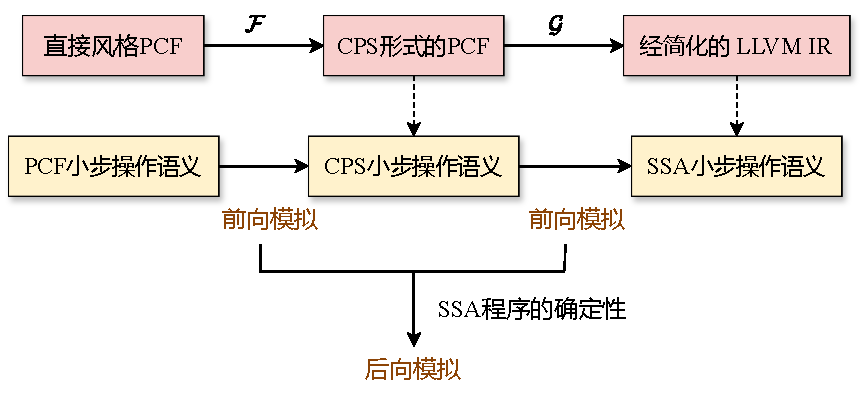
\includegraphics[width=0.8\linewidth]{figures/extracts.drawio.pdf}
    \caption{CPS到SSA基于模拟技术的验证}\label{extracts}
\end{figure}

其中,进行CPS转换时程序内部执行步骤遵循的是多步模拟,如图~\ref{plus}所示。
我们首先定义了直接风格PCF程序状态与CPS程序状态之间的匹配关系$\sim$。
PCF源程序经过一步转换,CPS可以在经过一步或多步转换后再次与之状态匹配。
在CPS转换中,我们不需要考虑无限驻留问题,因为目标程序至少需要走一步。

\begin{figure}[htbp]
    \centering
    \vspace{2ex}
    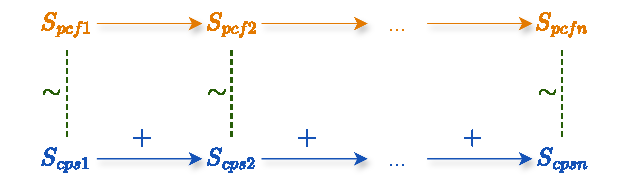
\includegraphics[width=0.75\linewidth]{figures/plus.drawio.pdf}
    \caption{PCF到CPS的多步模拟}\label{plus}
\end{figure}

对于CPS到SSA的转换,程序内部执行步骤遵循的是星形模拟,如图~\ref{star}所示。
我们同样需要为CPS程序和SSA程序定义了程序状态之间的匹配关系$\sim$。
CPS源程序经过一步转换,SSA程序可以在经过零步,一步或多步转换后再次与之状态匹配。
正如第~\ref{sec:compcertbackend}节中所言,星型模拟在目标程序进行零步转换仍然匹配时,
可能会出现无限驻留问题。因此,我们为CPS程序定义了度量函数,来防止出现星形模拟中的无限驻留问题。
如图~\ref{stutter}所示,当CPS程序进行一步转换时,SSA程序在原地驻留。
那么,如果CPS程序无限地进行这一步转换,它就会发散,而目标SSA程序始终驻留。
这样一来,源程序和目标程序的行为就不一致了。
所以,为了防止出现这种情况,我们为CPS程序状态定义了递减的度量函数。
度量函数的具体设计及作用将在第~\ref{sec:cpsssaforward}节中详述。

\begin{figure}[htbp]
    \centering
    \vspace{2ex}
    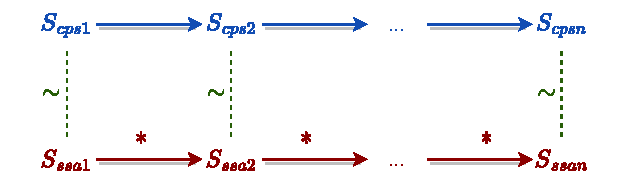
\includegraphics[width=0.75\linewidth]{figures/star.drawio.pdf}
    \caption{CPS到SSA的星型模拟}\label{star}
\end{figure}

\begin{figure}[htbp]
    \centering
    \vspace{2ex}
    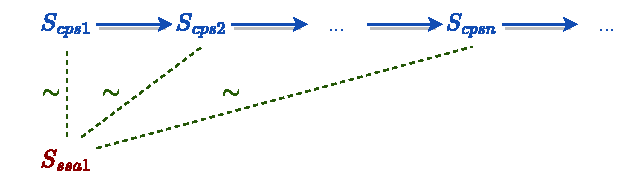
\includegraphics[width=0.75\linewidth]{figures/stutter.drawio.pdf}
    \caption{CPS到SSA可能出现的无限驻留问题}\label{stutter}
\end{figure}

将两步前向模拟组合起来可以得到从PCF源程序到SSA程序的前向模拟。
我们还证明了SSA程序的确定性,即同一个终止的SSA程序返回值是唯一确定的。
利用SSA程序的确定性和前向模拟性质,我们证明了PCF到SSA的后向模拟,
即SSA程序的行为是可接受的PCF程序行为。
这样,我们就验证了从PCF到SSA的核心编译过程的正确性。

完成了这样一个核心编译步骤经验证的基于SSA的PCF语言编译器,我们就用形式化的方法
将CPS与SSA联系在了一起,并为高可靠函数式编译器与主流编译器基础设施的连接提供了基础。
在接下来的两章中,我们将分别详细介绍关键编译步骤的转换算法和其语义保存性质的形式化验证。
该函数式编译器的具体代码实现将在第\ref{ch:implement}章中介绍。
% !TEX root = ../main.tex

\chapter{CPS到SSA中间语言的转换算法} \label{ch:trans}

在本章中,我们首先定义了CPS到SSA转换算法的源语言和目标语言,
给出了它们的语法及语义,然后详细介绍了该转换算法的设计和转换规则。
为了得到CPS形式的源语言,我们还介绍了将直接风格PCF程序进行CPS转换的算法。
我们还使用示例程序详细演示了这两个转换算法的工作流程。

\section{源语言:CPS形式的PCF语言} \label{sec:cps}

如第\ref{sec:overview}章中所述,PCF是一种被广泛应用于研究的函数式语言~\cite{plotkin1977lcf}。
在本节中,我们定义了直接风格和CPS形式PCF语言的语法和小步操作语义。
我们还描述了将直接风格PCF程序转换为CPS形式的算法。

\subsection{源语言的语法和语义}

本文中介绍的PCF语言来自Dowek和L{'e}vy的工作~\cite{dowek2010introduction}。
它包括基本的$\lambda$-演算、算术运算表达式、条件表达式和不动点(Fixed Point)。PCF及其CPS形式的语法定义如图~\ref{pcfsyntax}所示。

\begin{figure}[htbp]
        \centering
        \begin{subfigure}[b]{0.4\textwidth}
            \flushright
        \begin{equation}
            \nonumber
            \begin{aligned}
                op\, := &\; +\; |\; -\; | \; \times \; |\; \div \\
                t\, := &\; i\; |\; x\; |\; t_1\; t_2\; |\; \mathbf{ifz}\; t_1\; t_2\; t_3 \\
                & |\; op\; t_1\; t_2 \\
                & |\; \mathbf{let}\; x=t_1\; \mathbf{in}\; t_2 \\
                & |\; \mathbf{fix}\; f\; x\; t
            \end{aligned}
        \end{equation}
        \caption{直接风格的PCF语言语法}\label{directpcf}
        \end{subfigure}
       % \hfill
        \begin{subfigure}[b]{0.5\textwidth}
            \flushleft
        \begin{equation}
            \nonumber
            \begin{aligned}
                v\, := &\; i\; |\; x \\
                t\, := &\; \mathbf{letval}\; x=v\; \mathbf{in}\; t\; |\; k\; v\; |\; \mathbf{ifz}\; v\; t_1\; t_2 \\
                & |\; f\; k\; v\; |\; \mathbf{letop}\; x=op\; x_1\; x_2\; \mathbf{in}\; t \\
                & |\; \mathbf{letcont}\; k\; x=t_1\; \mathbf{in}\; t_2 \\
                & |\; \mathbf{letfun}\; f\; k\; x=t_1\; \mathbf{in}\; t_2 
            \end{aligned}
        \end{equation}
        \caption{CPS形式的PCF语言语法}\label{cpspcf}
    \end{subfigure}
    \caption{PCF语言语法}\label{pcfsyntax}
    \end{figure}

最基本的PCF代码项(Term)包含自然数$i$和变量$x$。将代码项$t_1$应用到代码项$t_2$上表示为$t_1\; t_2$。
我们使用$\mathbf{let}\; x = t_1\; \mathbf{in}\; t_2$表示在$t_2$中将变量$x$替换为$t_1$的值。
PCF中的条件表达式记作$\mathbf{ifz}\; t_1\; t_2\; t_3$。如果$t_1$的值为0,则整个代码项规约到$t_2$。
否则,它将规约到$t_3$。PCF中的不动点代码项是$\mathbf{fix}\; f\; x\; t$,其中$t$中可能出现$f$。
例如,图~\ref{factpcf}中展示了使用直接风格的PCF实现阶乘功能并应用到参数2的程序。

CPS形式的PCF语言遵循Kennedy提出的CPS风格函数式程序结构~\cite{kennedy2007compiling}。
值$v$在CPS项中可以通过$\mathbf{letval}\; x = v\; \mathbf{in}\; t$语句引入。$k\; v$将延续(Continuation)$k$应用于参数$v$。
$f\; k\; v$将函数$f$应用于参数$v$,并传递延续变量$k$以接受此调用返回的结果。
语句$\mathbf{letop}\; x = op\; x_1\; x_2\; \mathbf{in}\; t$将变量$x$在项$t$中绑定为该二元运算的结果。
通过$\mathbf{letcont}\; k\; x = t_1\; \mathbf{in}\; t_2$引入局部延续(Local Continuation)$k$,其中$t_1$是延续$k$的延续体(Body)。
$\mathbf{letfun}\; f\; k\; x = t_1\; \mathbf{in}\; t_2$构造一个返回延续(Return Continuation)为$k$的函数$f$。
图~\ref{factcps}描述了CPS形式的PCF语言中阶乘函数的实现及对参数2的应用,其中每个计算步骤都是被显式命名的。
可以看到,顶层延续变量$k_{init}$接受整个程序返回的结果,并由其上下文绑定。

\begin{figure}[htbp]
        \centering
        \begin{subfigure}[b]{0.3\textwidth}
            \flushright
        % \small
        \begin{equation}
            \nonumber
            \begin{aligned}
            & (\mathbf{fix}\; fact\; x \\
            & \quad \mathbf{ifz}\; x\; 1 \\
            & \quad\quad (x*(fact\; (x-1)))) \\
            & 2
            \end{aligned}
        \end{equation}
        \caption{直接风格的PCF阶乘程序}\label{factpcf}
        \end{subfigure}
        \begin{subfigure}[b]{0.68\textwidth}
            \flushleft
            % \small
        \begin{equation}
            \nonumber
            \begin{aligned}
            & \mathbf{letfun}\; fact\; k\; x = (\mathbf{ifz}\; x\; (\mathbf{letval}\; x_1=1\; \mathbf{in}\; (k\; x_1))\\
            & \quad (\mathbf{letval}\; x_2=1\; \mathbf{in}\; (\mathbf{letop}\; x_4=x-x_2\; \mathbf{in} \\
            & \quad\quad \mathbf{letcont}\; k_1\; z= (\mathbf{letop}\; x_3=x*z\; \mathbf{in}\; (k\; x_3))\\
            & \quad\quad\quad  \mathbf{in}\; fact\; k_1\; x_4)))\; \mathbf{in} \\
            & (\mathbf{letval}\; x_5=2\; \mathbf{in}\; (\mathbf{letcont}\; k_2\; y=k_{init}\; y\; \mathbf{in}\; (fact\; k_2\; x_5))) \\
            \end{aligned}
        \end{equation}
        \caption{CPS形式的PCF阶乘程序}\label{factcps}
        \end{subfigure}
    \caption{使用PCF语言实现阶乘程序}\label{factpcfcps}
    \end{figure}

接下来,我们需要为以上所介绍的PCF语言提供小步操作语义。
$S\rightarrow S'$表示执行一步操作可以使程序从初始状态$S$到达状态$S'$。
在直接风格的PCF程序中,程序状态之间的转换步骤表示为:
\begin{equation}
(t_{pcf},ctx)\rightarrow (t'_{pcf},ctx').
\end{equation}
$t_{pcf}$表示的是正在被求值(Evaluate)的表达式的PCF代码项。
$ctx$是一个包含代码项序列的上下文(Context),用于在当前$t_{pcf}$的求值完成后进行下一步执行操作。
当$ctx = ctx_{stop}$时,程序执行在$t_{pcf}$求值完成后即可结束。否则,当$ctx = ctx_{seq}\; t\; ctx$,
表示$t_{pcf}$的值将作为后续代码项$t$的参数,程序继续执行。经过一步转换之后,
新的程序状态包含了更新后的PCF代码项$t'_{pcf}$和新的上下文$ctx'$。转换规则如图~\ref{pcfopsem}所示。

$\mathbf{let}$表达式在$t_2$中用代码项$t_1$的值替换变量$x$。
因此,我们首先对$t_1$进行求值并将当前求值完成后下一步需要处理的代码项追加在上下文$ctx$中。
然后,在得到$t_1$的值后,我们将$t_2$中的变量$x$进行替换。当将不动点应用于代码项$t_2$时,
也是进行类似的操作。先将不动点放入上下文中,当$t_2$的值计算完毕后,将用它来替换不动点中的参数$x$,然后计算继续进行。
对于$\mathbf{ifz}$条件语句,我们求出$t_1$的值$n$,并根据$n$是否为0来确定下一步规约操作。

\begin{figure}[t]
    \centering
    \setlength{\jot}{10pt}
    \begin{gather*}
        \tag*{ps\_let\_app} \displaystyle{\frac{t_{pcf}=(\mathbf{let}\; x = t_1\; \mathbf{in}\; t_2)} {(t_{pcf},\; ctx)\rightarrow (t_1,\; ctx_{seq}\; t_{pcf}\; ctx)}} \\
        \tag*{ps\_let\_abs} \displaystyle{\frac{t_1\; is\; a\; value\quad t_3=(\mathbf{let}\; x = t_1\; \mathbf{in}\; t_2)} {(t_1,\; ctx_{seq}\; t_3\; ctx)\rightarrow (t_2 [t_1/x],\; ctx)}} \\
        \tag*{ps\_if\_zero} \displaystyle{(\mathbf{ifz}\; 0\; t_2\; t_3,\; ctx)\rightarrow (t_2,\; ctx)} \\
        \tag*{ps\_if\_notzero} \displaystyle{\frac{n \neq 0}{(\mathbf{ifz}\; n\; t_2\; t_3,\; ctx)\rightarrow (t_3,\; ctx)}} \\
        \tag*{ps\_if\_app} \displaystyle{\frac{t_{pcf}=(\mathbf{ifz}\; t_1\; t_2\; t_3)} {(t_{pcf},\; ctx)\rightarrow (t_1,\; ctx_{seq}\; t_{pcf}\; ctx)}} \\
        \tag*{ps\_if\_abs} \displaystyle{\frac{v\; is\; a\; value\quad t_3=(\mathbf{ifz}\; t_1\; t_2\; t_3)} {(v,\; ctx_{seq}\; t_3\; ctx)\rightarrow (t_3 [v/t_1],\; ctx)}} \\
        \tag*{ps\_fix\_app} \displaystyle{\frac{t_{pcf}=((\mathbf{fix}\; f\; x\; t_1)\; t_2)} {(t_{pcf},\; ctx)\rightarrow (t_2,\; ctx_{seq}\; (\mathbf{fix}\; f\; x\; t_1)\; ctx)}} \\
        \tag*{ps\_fix\_abs} \displaystyle{\frac{t_2\; is\; a\; value\quad t_3=(\mathbf{fix}\; f\; x\; t_1)} {(t_2,\; ctx_{seq}\; t_3\; ctx)\rightarrow (t_1 [t_2/x,t_3/f],\; ctx)}} \\
        \tag*{ps\_op\_fst} \displaystyle{(op\; t_1\; t_2,\; ctx)\rightarrow (t_1,\; ctx_{seq}\; (op\; t_1\; t_2,\; ctx)\; ctx)} \\
        \tag*{ps\_op\_snd} \displaystyle{\frac{v_1\; is\; a\; value\quad t_3=(op\; t_1\; t_2,\; ctx)} {(v_1,\; ctx_{seq}\; t_3\; ctx)\rightarrow (t_2,\; ctx_{seq}\; (op\; v_1\; t_2)\; ctx)}} \\
        \tag*{ps\_op\_cal} \displaystyle{\frac{v_1,\; v_2\; are\; values\quad n=\mathbf{eval}_{op}\; op\; v_1\; v_2}{(v_2,\; ctx_{seq}\; (op\; v_1\; t_2)\; ctx)\rightarrow (n,\; ctx)}} \\
    \end{gather*}  
    \caption{直接风格的PCF语言小步操作语义转换规则} \label{pcfopsem}
\end{figure}

% \begin{figure}[t]
%     \centering
%     \begin{subfigure}[t]{0.43\textwidth}
%         \setlength{\jot}{10pt}
%         \begin{gather*}
%             \displaystyle{\frac{t_{pcf}=(\mathbf{let}\; x = t_1\; \mathbf{in}\; t_2)} {(t_{pcf},\; ctx)\rightarrow (t_1,\; ctx_{seq}\; t_{pcf}\; ctx)}} \\
%             \displaystyle{\frac{t_1\; is\; a\; value\quad t_3=(\mathbf{let}\; x = t_1\; \mathbf{in}\; t_2)} {(t_1,\; ctx_{seq}\; t_3\; ctx)\rightarrow (t_2 [t_1/x],\; ctx)}} \\
%             \displaystyle{\frac{v\; is\; a\; value\quad t_3=(\mathbf{ifz}\; t_1\; t_2\; t_3)} {(v,\; ctx_{seq}\; t_3\; ctx)\rightarrow (t_3 [v/t_1],\; ctx)}} \\
%             \displaystyle{\frac{t_{pcf}=(\mathbf{ifz}\; t_1\; t_2\; t_3)} {(t_{pcf},\; ctx)\rightarrow (t_1,\; ctx_{seq}\; t_{pcf}\; ctx)}} \\
%             \displaystyle{(\mathbf{ifz}\; 0\; t_2\; t_3,\; ctx)\rightarrow (t_2,\; ctx)} \\
%             \displaystyle{\frac{n \neq 0}{(\mathbf{ifz}\; n\; t_2\; t_3,\; ctx)\rightarrow (t_3,\; ctx)}} \\
%         \end{gather*}
%     \end{subfigure}
%     \begin{subfigure}[t]{0.55\textwidth}
%         \setlength{\jot}{10pt}
%         \begin{gather*}
%             \displaystyle{\frac{t_{pcf}=((\mathbf{fix}\; f\; x\; t_1)\; t_2)} {(t_{pcf},\; ctx)\rightarrow (t_2,\; ctx_{seq}\; (\mathbf{fix}\; f\; x\; t_1)\; ctx)}} \\
%             \displaystyle{\frac{t_2\; is\; a\; value\quad t_3=(\mathbf{fix}\; f\; x\; t_1)} {(t_2,\; ctx_{seq}\; t_3\; ctx)\rightarrow (t_1 [t_2/x,t_3/f],\; ctx)}} \\
%             \displaystyle{(op\; t_1\; t_2,\; ctx)\rightarrow (t_1,\; ctx_{seq}\; (op\; t_1\; t_2,\; ctx)\; ctx)} \\
%             \displaystyle{\frac{v_1\; is\; a\; value\quad t_3=(op\; t_1\; t_2,\; ctx)} {(v_1,\; ctx_{seq}\; t_3\; ctx)\rightarrow (t_2,\; ctx_{seq}\; (op\; v_1\; t_2)\; ctx)}} \\
%             \displaystyle{\frac{v_1,\; v_2\; are\; values\quad n=\mathbf{eval}_{op}\; op\; v_1\; v_2}{(v_2,\; ctx_{seq}\; (op\; v_1\; t_2)\; ctx)\rightarrow (n,\; ctx)}} \\
%         \end{gather*}
%     \end{subfigure}   
%     \caption{直接风格的PCF语言小步操作语义转换规则} \label{pcfopsem}
% \end{figure}

CPS形式的PCF语言的小步操作语义表示的推导规则形如
\begin{equation}
(t_{cps},loc_{cps})\rightarrow(t'_{cps},loc'_{cps}).
\end{equation}
同样的,$t_{cps}$是正在被计算的CPS代码项,$loc_{cps}$是从延续变量名或函数名到引入它们的代码项的映射(Mapping)。
$t'_{cps}$和$loc'_{cps}$分别是更新后的CPS代码项和映射。
CPS形式的PCF语言的小步操作语义转换规则如图~\ref{cpsopsem}所示。
$\mathbf{letval}$表达式可以将新的值引入代码项$t$,我们只需要在$t$中用$v$替换变量$x$。
对于代码项$(\mathbf{letcont}\; k\; x=t_1\; \mathbf{in}\; t_2)$,
首先对$t_2$求值并更新$loc_{cps}$,添加从延续变量$k$到该代码项的映射。
我们使用$loc_{cps}\; [k\mapsto t_{cps}]$这种标记来表示对映射$loc_{cps}$的更新操作。
当把延续$k$应用于值$v$时(用$k\; v$表示),由于$t_1$是延续$k$的延续体,我们将$t_1$中的变量$x$替换为$v$。
$\mathbf{letfun}$代码项的规约与之类似,当我们遇到$\mathbf{letfun}$结构时,我们会更新从$f$到该项的映射。
当我们将延续$k_0$和变量$x_0$作为参数传递给$f$时,我们分别用$k_0$和$x_0$替换函数体$t_1$中的$k$和$x$。

\begin{figure}[htbp]
    \centering
    \setlength{\jot}{10pt}
    \centering
    \begin{gather*}
        \tag*{cs\_val} \displaystyle{\frac{t_{cps}=(\mathbf{letval}\; x=v\; \mathbf{in}\; t)} {(t_{cps},\; loc_{cps})\rightarrow (t [v/x],\; loc_{cps})}} \\
        \tag*{cs\_if\_zero} \displaystyle{\frac{t_{cps}=(\mathbf{ifz}\; 0\; t_1\; t_2)} {(t_{cps},\; loc_{cps})\rightarrow (t_1,\; loc_{cps})}} \\
        \tag*{cs\_if\_notzero} \displaystyle{\frac{t_{cps}=(\mathbf{ifz}\; n\; t_1\; t_2)\quad n \neq 0} {(t_{cps},\; loc_{cps})\rightarrow (t_2,\; loc_{cps})}} \\
        \tag*{cs\_cont\_app} \displaystyle{\frac{loc_{cps}\; k = (\mathbf{letcont}\; k\; x=t_1\; \mathbf{in}\; t_2)}{(k\; v,\; loc_{cps})\rightarrow (t_1 [v/x],\; loc_{cps})}} \\
        \tag*{cs\_cont} \displaystyle{\frac{t_{cps}=(\mathbf{letcont}\; k\; x=t_1\; \mathbf{in}\; t_2)} {(t_{cps},\; loc_{cps})\rightarrow (t_2,\; loc_{cps}\; [k\mapsto t_{cps}])}} \\
        \tag*{cs\_letop} \displaystyle{\frac{t_{cps}=(\mathbf{letop}\; x=op\; v_1\; v_2\; \mathbf{in}\; t)}{(t_{cps},\; loc_{cps})\rightarrow (t [(\mathbf{eval}_{op}\; op\; v_1\; v_2)/x],\; loc_{cps})}} \\
        \tag*{cs\_fun} \displaystyle{\frac{t_{cps}=(\mathbf{letfun}\; f\; k\; x=t_1\; \mathbf{in}\; t_2)} {(t_{cps},\; loc_{cps})\rightarrow (t_2,\; loc_{cps}\; [f\mapsto t_{cps}])}} \\
        \tag*{cs\_fun\_app} \quad \displaystyle{\frac{loc_{cps}\; f = (\mathbf{letfun}\; f\; k\; x=t_1\; \mathbf{in}\; t_2)}{(f\; k_0\; x_0,\; loc_{cps})\rightarrow (t_1 [x_0/x, k_0/k],\; loc_{cps})}}
    \end{gather*}   
    \caption{CPS形式的PCF语言小步操作语义转换规则}\label{cpsopsem}
\end{figure}

\subsection{直接风格PCF语言的CPS转换} \label{sec:cpstrans}

如第\ref{sec:bg_cps}节中所述,函数式语言的编译器通常会将直接风格的源程序转换为CPS形式,
即进行CPS转换(CPS Transformation)。本节中,我们将介绍把PCF源程序转换为CPS形式的编译算法。
该算法遵循CPS转换的一般模式~\cite{plotkin1975call,danvy2007one},根据计算的层次顺序递归地解构处理PCF代码项。
例如,如果PCF代码项$t$的计算步骤可以有序地分为对$t_1$和$t_2$的计算,
那么我们就可以把对$t_2$进行转换得到的CPS代码项放入之后要处理的参数中,并在下一步中直接开始处理$t_1$。 

转换过程由图~\ref{algo:cpstrans}中的函数$\mathcal{F}_{proc}$描述,它使用了一个更加广义的转换函数$\mathcal{F}$。
函数$\mathcal{F}$的输入和输出分别表示为$(t_{pcf}, l_v, \kappa)$和$t_{cps}$。
$t_{pcf}$是待转换的PCF程序。$\kappa$的结构表示为$\lambda x. t'_{cps}$,
代表了当前代码项被归约到一个值后要被应用的CPS代码项(延续)。$t_{cps}$是其生成的CPS程序。
在我们的CPS转换算法中,变量使用有名字的字符串名称。$l_v$是已经被使用的变量列表,
新生成的名称不能与$l_v$中的名称冲突。例如,使用图~\ref{algo:cpstrans}中的规则(3)对$t_1\; t_2$进行转换,
生成的新变量$k,\, x,\, y,\, z$必须不能已经存在于$l_v$中。该步转换之后,它们被添加到$l_v$中。
为了简化转换规则,我们没有在图中的算法里写出使用$l_v$指定生成新变量的具体操作。
它所做的其实是通过维护最新生成的变量的下标,来选择最小未使用的正数作为新变量的下标。
在初始状态中,要转换的PCF程序即为源程序$t_{pcf}$,新生成的名称只有顶层延续变量的名字$k_{init}$。
此时参数$\kappa$为$\lambda x. (k_{init}\; x)$,表示它接受整个生成的$t_{cps}$程序的值。
因此,应用$k_{init}$的值将是程序的最终结果。

\begin{figure}[t]
    \centering
    \vspace{2ex}
    % \small
    % \setlength{\jot}{10pt}
    \begin{algorithm}[H]
        \caption{CPS转换}
        \SetAlgoLined
        $\mathcal{F}_{proc}:\quad \mathbf{Input:}\; t_{pcf}\quad \mathbf{Output:}\; t_{cps}$\\
        $\mathcal{F}_{proc}(t_{pcf})\coloneqq \mathbf{\mathcal{F}}(t_{pcf}, [k_{init}], \lambda x. (k_{init}\; x))$\\
        \vspace*{0.5em}
        $\mathcal{F}:\quad \mathbf{Input:}\; t_{pcf},\; l_v,\; \kappa \quad \mathbf{Output:}\; t_{cps}$\\ 
        $(1).\; \mathbf{\mathcal{F}}(i, l_v, \kappa) \coloneqq \textcolor{blue}{\mathbf{letval}\; x= i\; \mathbf{in}\; \kappa(x)} $ \\
        $(2).\; \mathbf{\mathcal{F}}(x, l_v, \kappa) \coloneqq \kappa(x) $ \\
        $(3).\; \mathbf{\mathcal{F}}(t_1\; t_2, l_v, \kappa) \coloneqq \mathbf{\mathcal{F}}(t_1, l'_v,\lambda x. \mathbf{\mathcal{F}}(t_2, l'_v, \lambda y. (\textcolor{blue}{\mathbf{letcont}\; k\; z=\kappa(z)\; \mathbf{in}\; (x\; k\; y)})))$ \\
        $\quad\quad \mathtt{where}\; l'_v = l_v \doubleplus [k;x;y;z]$ \\
        $(4).\; \mathbf{\mathcal{F}}(\mathbf{ifz}\; t_1\; t_2\; t_3, l_v, \kappa) \coloneqq \mathbf{\mathcal{F}}(t_1, l'_v, \lambda x. (\textcolor{blue}{\mathbf{ifz}\; x\; \mathbf{\mathcal{F}}(t_2, l'_v, \kappa)\; \mathbf{\mathcal{F}}(t_3, l'_v, \kappa)}))  $ \\
        $\quad\quad \mathtt{where}\; l'_v = l_v \doubleplus [x]$ \\
        $(5).\; \mathbf{\mathcal{F}}(op\; t_1\; t_2, l_v, \kappa) \coloneqq \mathbf{\mathcal{F}}(t_1, l'_v,\lambda x.\mathbf{\mathcal{F}}(t_2, l'_v, \lambda y. (\textcolor{blue}{\mathbf{letop}\; z=op\; x\; y\; \mathbf{in}\; \kappa(z)}))) $ \\
        $\quad\quad \mathtt{where}\; l'_v = l_v \doubleplus [x;y;z]$ \\
        $(6).\; \mathbf{\mathcal{F}}(\mathbf{let}\; x=t_1\; \mathbf{in}\; t_2, l_v, \kappa) \coloneqq \mathbf{\mathcal{F}}(t_1, l_v, \lambda x. \mathbf{\mathcal{F}}(t_2, l_v, \kappa)) $ \\
        $(7).\; \mathbf{\mathcal{F}}(\mathbf{fix}\; f\; x\; t, l_v, \kappa) \coloneqq \textcolor{blue}{\mathbf{letfun}\; f\; k\; x= \mathbf{\mathcal{F}}(t, l'_v, \lambda y. (k\; y))\; \mathbf{in}\; \kappa(f)}$ \\
        $\quad\quad \mathtt{where}\; l'_v = l_v \doubleplus [k;y]$
    \end{algorithm}
    \caption{CPS转换算法}\label{algo:cpstrans}
\end{figure}

接下来,我们将以图~\ref{factpcfcps}中的直接风格与CPS形式PCF程序为例,说明以上CPS转换算法是如何将
图~\ref{factpcf}中的程序转换为图~\ref{factcps}中的程序。说明过程中我们会略去新变量名的生成方法
和$l_v$参数的维护,因为它们始终遵循同样的方法,不需再逐步描述。以下说明中已生成变量名参数均记为$l_v$。

\begin{enumerate}
    \item 首先对CPS源程序应用图~\ref{algo:cpstrans}中的规则(3),下一步需要处理的PCF程序变为
        子代码项$\mathbf{fix}\; fact\; x\; \dots$,参数$\kappa $从初始状态时的$\lambda x. (k_{init}\; x)$变为
        $\lambda x. \mathbf{\mathcal{F}}(2, l_v, \lambda z. $ \\ $(\mathbf{letcont}\; k_2\; y=k_{init}\; y\; \mathbf{in}\; (x\; k_2\; z)))$。
    \item 先对参数$\kappa $中的$\mathbf{\mathcal{F}}$进行处理。根据规则(1),我们添加$\mathbf{letval}$结构并用$x_5$替换绑定变量$z$,它转换为
        $\mathbf{letval}\; x_5 = 2\; \mathbf{in}\; (\mathbf{letcont}\; k_2\; y=k_{init}\; y\; \mathbf{in}\; (x\; k_2\; x_5))$。
        我们将其记为$t_{cps1}$,那么当前的参数$\kappa $就是$\lambda x. t_{cps1}$。
    \item 根据规则(7)处理$\mathbf{fix}$代码项,$\kappa(fact)$就是将$t_{cps1}$中的绑定变量名$x$替换为$fact$,
    把$\mathbf{fix}$代码项的函数体部分记为$t_{cps2}$,CPS转换的目标程序变为:
    \begin{equation}
        \nonumber
        \begin{aligned}
        & \mathbf{letfun}\; fact\; k\; x = \mathbf{\mathcal{F}}(t_{cps2}, l_v, \lambda y. (k\; y))\; \mathbf{in} \\
        & \quad (\mathbf{letval}\; x_5=2\; \mathbf{in}\; (\mathbf{letcont}\; k_2\; y=k_{init}\; y\; \mathbf{in}\; (fact\; k_2\; x_5))) \\
        \end{aligned}
    \end{equation}
    \item 接下来的任务就是求出$\mathbf{\mathcal{F}}(t_{cps2}, l_v, \lambda y. (k\; y))$。
        由于$t_{cps2}$是一个条件表达式,我们使用规则(4)处理它。
        将当前的$\kappa$参数记为$\kappa_1$,将PCF子代码项$(x*(fact\; (x-1)))$记为$t_{cps3}$,目标转换为
        $\mathbf{\mathcal{F}}(x, l_v, \lambda y. (\mathbf{ifz}\; y\; \mathbf{\mathcal{F}}(1, l_v, \kappa_1)\; \mathbf{\mathcal{F}}(t_{cps3}, l_v, \kappa_1)))$。
        按照规则(2),待处理PCF为变量时可以直接把当前的参数$\kappa$应用到变量$x$上。对于$\mathbf{\mathcal{F}}(1, l_v, \kappa_1)$可以使用规则(1)。
        目标转换为$\mathbf{ifz}\; x\; \mathbf{letval}\; x_1 = 1\; \mathbf{in}\; (k\; x_1)\; \mathbf{\mathcal{F}}(t_{cps3}, $ \\ $l_v, \kappa_1)$。
    \item 问题转换为求出$\mathbf{\mathcal{F}}(t_{cps3}, l_v, \kappa_1)$。对于二元算术运算,我们按照规则(5)进行处理。
        由于第一个操作数$x$是一个变量,我们可以直接用它来替换新的参数$\kappa$中的绑定变量。
        待求的程序变为$\mathbf{\mathcal{F}}(fact\; (x-1), l_v, \lambda m. (\mathbf{letop}\; x_3=x*m\; \mathbf{in}\; k\; x_3))$。
        $fact$是函数名,同时也是变量名。将其应用到$(x-1)$上可以使用转换规则(3)。
    \item 由于规则(1)、(2)、(3)和(5)在前几步的转换中都已经使用过,之后的转换步骤还是运用这几条规则,在此不再详述。
        最终,我们得到的CPS目标程序就是图~\ref{factcps}所示的程序。
\end{enumerate}

\section{目标语言:类似LLVM IR的SSA语言}

本文中使用的目标SSA语言是一种简化版本的LLVM IR,保留了其最基本的程序结构层次。
在本节接下来的内容中,我们将定义它的语法和小步操作语义,并讨论对SSA程序中自由变量的处理和避免。

\subsection{目标语言的语法和语义}

\begin{figure}[htbp]
    \centering
    \begin{equation}
        \nonumber
        \begin{aligned}
            l &\coloneqq string & v &\coloneqq i\; |\; x & r &\coloneqq \mathbf{ret}\; v\; |\; \mathbf{br_{uc}}\; l\; |\; \mathbf{br_c}\; v\; l_1\; l_2 \\
            \phi_a &\coloneqq (l,\; v) & \phi &\coloneqq x = \overline{\phi_a} &  c &\coloneqq v\; |\; op\; v_1\; v_2\; |\; \mathbf{icmp}\; v_1\; v_2\; |\; \mathbf{call}\; x\; v \\
            a &\coloneqq x = c; & b &\coloneqq l:\; \overline{\phi}\; \overline{a}\; r & f &\coloneqq \mathbf{define}\; l_1(l_2)\; \overline{b} \quad\quad\quad t \coloneqq \overline{f} \\
        \end{aligned}
    \end{equation}
    \caption{SSA目标语言的语法}\label{synssa}
\end{figure}

我们使用的目标SSA语言的语法定义如图~\ref{synssa}所示。
顶层的翻译单元(Translation Unit)$t$由一系列函数定义组成。
一个函数$f$包含函数名$l_1$、参数$l_2$和一系列基本代码块$\overline{b}$。
一个基本代码块$b$由它的标签$l$、$\overline{\phi}$节点序列、指令$\overline{a}$序列和一个终止指令(Terminator)$r$组成。
一条指令$a$将命令$c$的值赋给变量$x$。$c$包括值$v$、二元运算表达式、比较两个值是否相等的命令和函数调用。
终止指令包括$\mathbf{ret}$和$\mathbf{br}$,分别用于表示函数返回和块之间的跳转。
作为示例程序,图~\ref{factssa}展示了SSA中的阶乘函数与2的阶乘。

\begin{figure}[ht]
    \centering
    \begin{equation}
        \nonumber
        \begin{aligned}
            & \mathbf{define}\; fact\; (x)\\
            & \quad b_1:\; b_0 = \mathbf{icmp}\; x\; 0;\; \mathbf{br_c}\; b_0\; t_0\; f_0; \\
            & \quad t_0:\; x_1 = 1;\; r_{t0} = x_1;\; \mathbf{ret}\; r_{t0}; \\
            & \quad f_0:\; x_2 = 1;\; x_4 = x - x_2;\; z = \mathbf{call}\; fact\; x_4;\; \mathbf{br_{uc}}\; k_1; \\
            & \quad k_1:\; x_3 = x*z;\; r_{k1} = x_3;\; \mathbf{ret}\; r_{k1}; \\
            & \mathbf{define}\; main\; ( )\\
            & \quad b_1:\; x_5 = 2;\; y = \mathbf{call}\; fact\; x_5;\; \mathbf{br_{uc}}\; k_2;\\
            & \quad k_2:\; r_{k2} = y;\; \mathbf{ret}\; r_{k2};
        \end{aligned}
    \end{equation}
    \caption{SSA语言中的阶乘程序}\label{factssa}
\end{figure}

目标SSA语言的小步操作语义规则表示为
\begin{equation}
(pc, ppc, loc_{ssa}, s_{ssa}) \rightarrow (pc', ppc', loc'_{ssa}, s'_{ssa}).
\end{equation}
$pc$是程序计数器(Program Counter),用于定位当前指令,由三个元素$(l_{f}, l_b, n)$组合而成。
其中,$l_{f}$是当前函数标签,$l_b$是当前基本代码块标签,$n$表示基本块中指令的位置。
可以使用$\mathbf{code}_{at}\; pc$获取$pc$位置处的指令。$ppc$存储了上一个块中进行跳转之前的程序计数器值,
以便对$\phi$-节点进行求值。$loc_{ssa}$是变量名到它们的值的映射。
我们在堆栈$s_{ssa}$中保留调用当前函数的指令的程序计数器,以便在当前函数返回时能够返回到调用时的位置。

SSA语言的操作语义转换规则如图~\ref{ssaopsem}所示。
第一条规则描述了函数调用的程序状态转换。
控制流跳转到函数$f$的开头,并将函数返回地址存储在$s_{ssa}$中。
$\mathbf{arg}\; f$表示获取函数$f$的参数,$loc_{ssa}\; [x\mapsto v_0]$表示把从$x$到$v_0$的映射添加到$loc_{ssa}$中。
例如,在图~\ref{factssa}中,当主函数调用$fact$函数时,按照图~\ref{ssaopsem}中的第一条规则,
程序状态从$((main,b_1,1),\, (main,empty,1),\, loc_{ssa},\, s_{ssa})$ 
转换到$((fact,b_1,0),\, (main,b_1,1),\, loc_{ssa}$ \\ $[x\mapsto 2],\, \mathbf{push}\; s_{ssa}\; (main,b_1,1))$。
第二条规则定义了当前函数返回并将返回值传递给调用语句时发生的状态转换。
它从$s_{ssa}$的顶部取出程序计数器$npc$,存储返回值,并跳回该调用语句的位置。
对于$\phi$-节点,我们利用$ppc$提供的信息得到前驱基本块的标签,从而确定变量$x$被赋予的值是哪个版本。
二元算术运算语句、普通赋值语句和$\mathbf{icmp}$语句的处理方法类似,都是利用$loc_{ssa}$计算变量被赋予的具体值,并更新到映射中。
在我们的SSA程序中,变量被使用之前一定是被赋值过的,所以可以计算出这些语句等号右边表达式结果值。
对于无条件跳转和条件跳转语句,由于它们只是同一函数内不同基本代码块之间的跳转,我们只需求出新的基本块标签。
当然,在下一个程序状态中$ppc$就变成了当前状态的$pc$。

\begin{figure}[htbp]
    % \vspace*{-0.3cm}
    \centering
    % \small
    \setlength{\jot}{10pt}
    \begin{gather*}
        \tag*{ss\_call} \displaystyle{\frac{\mathbf{code}_{at}\; pc\; =\; (y=\mathbf{call}\; f\; v_0)\quad \mathbf{arg}\; f = x}
        {(pc,\; ppc,\; loc_{ssa},\; s_{ssa})\rightarrow ((f,b_1,0),\; pc,\; loc_{ssa}\; [x\mapsto v_0],\; \mathbf{push}\; s_{ssa}\; pc )}} \\
        % & \displaystyle{\frac{\mathbf{code}_{at}\; pc\; =\; id = phi,\quad n = \mathbf{eval}_{phi}\ phi\ ppc\ loc_{ssa} } {(pc,\; ppc,\; loc_{ssa},\; ploc_{ssa})\rightarrow (pc+1,\; ppc,\; loc_{ssa}\; id\mapsto n,\; ploc_{ssa})}} \\
        \tag*{ss\_ret} \displaystyle{\frac{\begin{matrix}\mathbf{code}_{at}\; pc\; =\; (\mathbf{ret}\; v)\quad pc.l_f \neq main\quad npc = \mathbf{top}\; s_{ssa}
        \\ \mathbf{code}_{at}\; npc\; =\; (x=\mathbf{call}\; f\; v_0)\end{matrix}} 
        {(pc,\; ppc,\; loc_{ssa},\; s_{ssa})\rightarrow (npc+1,\; pc,\; loc_{ssa}\; [x\mapsto v],\; \mathbf{pop}\; s_{ssa})}} \\
        \tag*{ss\_phi} \displaystyle{\frac{\mathbf{code}_{at}\; pc\; =\; (x=\overline{\phi_a})\quad n\; =\; \mathbf{eval}_{\phi}\ \overline{\phi_a}\ ppc}
            {(pc,\; ppc,\; loc_{ssa},\; s_{ssa})\rightarrow (pc+1,\; ppc,\; loc_{ssa}\; [x\mapsto n],\; s_{ssa})}} \\
        \tag*{ss\_op} \displaystyle{\frac{\mathbf{code}_{at}\; pc\; =\; (x=op\; v_1\; v_2)\quad n\; =\; \mathbf{eval}_{exp}\ loc_{ssa}\ op\; v_1\; v_2}
        {(pc,\; ppc,\; loc_{ssa},\; s_{ssa})\rightarrow (pc+1,\; ppc,\; loc_{ssa}\; [x\mapsto n],\; s_{ssa})}} \\
        \tag*{ss\_assign} \displaystyle{\frac{\mathbf{code}_{at}\; pc\; =\; (x=v)\quad n\; =\; v\; is\; value?\; v\; :\; (loc_{ssa}\; v)}
        {(pc,\; ppc,\; loc_{ssa},\; s_{ssa})\rightarrow (pc+1,\; ppc,\; loc_{ssa}\; [x\mapsto n],\; s_{ssa})}} \\
        \tag*{ss\_icmp} \displaystyle{\frac{\mathbf{code}_{at}\; pc\; =\; (x=\mathbf{icmp}\; v_1\; v_2)\quad \mathbf{if}\; (\mathbf{equal}_{val}\; loc_{ssa}\; v_1\; v_2)\; n=1\; \mathbf{else}\; n=0}
        {(pc,\; ppc,\; loc_{ssa},\; s_{ssa})\rightarrow (pc+1,\; ppc,\; loc_{ssa}\; [x\mapsto n],\; s_{ssa})}} \\
        \tag*{ss\_br\_uc} \displaystyle{\frac{\mathbf{code}_{at}\; pc\; =\; (\mathbf{br_{uc}}\; l)}
        {(pc,\; ppc,\; loc_{ssa},\; s_{ssa})\rightarrow ((pc.l_f, l, 0),\; pc,\; loc_{ssa},\; s_{ssa})}} \\
        \tag*{ss\_br\_c} \displaystyle{\frac{\mathbf{code}_{at}\; pc\; =\; (\mathbf{br_c}\; v\; l_1\; l_2)\quad \mathbf{if}\; (\mathbf{equal}_{val}\; loc_{ssa}\; v\; 0)\; l_n=l_1\; \mathbf{else}\; l_n=l_2}
        {(pc,\; ppc,\; loc_{ssa},\; s_{ssa})\rightarrow ((pc.l_f, l_n, 0),\; pc,\; loc_{ssa},\; s_{ssa})}}
    \end{gather*}
    \caption{目标SSA语言的小步操作语义转换规则}\label{ssaopsem}
\end{figure}

\subsection{含有自由变量的函数}

我们的目标SSA语言与LLVM IR之间的一个重要区别在于,$loc_{ssa}$是一个全局映射(Global Mapping),
我们允许函数包含未在该函数中定义的自由变量(Free Variables)。这样做是因为我们的源语言是带有自由变量的高阶函数。
典型的函数式语言编译器会对CPS程序使用闭包转换(Closure Conversion),将开放函数转换为闭包。
闭包转换的形式化验证已经得到广泛研究~\cite{paraskevopoulou2019closure,wang-esop2016}。
为简单起见,我们没有将闭包转换包含在我们的编译链中。我们的SSA语言支持闭包和开放函数,
并专注于CPS到SSA转换的本质。在接下来的内容中我们将讨论这一点。

\section{转换算法设计} \label{sec:cpsssatrans}

我们设计了将CPS形式的PCF程序转换为SSA程序的转换算法。本质上,该转换过程是一个递归函数,
它接受一个CPS代码项、一个SSA程序及其他信息作为其参数,不断将新的组件(例如基本代码块、指令等)
放入当前SSA程序的特定位置,并在递归地翻译CPS代码项时更新其他参数。
这些参数是确定新的组件具体内容及插入位置所必须的信息。
一旦整个CPS程序的翻译完成,所得到的SSA程序就是我们需要的转换后的目标SSA程序。

\begin{figure}[!ht]
    \centering
    \vspace{2ex}
    % \setlength{\jot}{10pt}
    \begin{algorithm}[H]
        \caption{CPS$\rightarrow $SSA 转换}
        \SetAlgoLined
        $\mathcal{G}_{proc}:\quad \mathbf{Input:}\; t_{cps}\quad \mathbf{Output:}\; t_{ssa}$\\
        $\mathcal{G}_{proc}(t_{cps})\coloneqq t_{ssa}  $\\
        $\quad\quad \mathtt{where}\; (t_{ssa}, n, loc) = \mathbf{\mathcal{G}}(t_{cps}, \mathbf{app}_b\; nil\; main, (main, b_1, 0), 0, loc_{empty}) $\\
        % $\quad\quad\quad\quad t_{ssa}$ \\
        \vspace*{0.5em}
        $ \mathbf{\mathcal{G}}:\quad \mathbf{Input:}\; t_{cps}, t_{ssa}, pc, n, loc\quad \mathbf{Output:}\; t'_{ssa}, n', loc' $ \\
        $ (1).\; \mathbf{\mathcal{G}}(\textcolor{blue}{\mathbf{letval}\; x=v\; \mathbf{in}\; t}, t_{ssa}, pc, n, loc) \coloneqq  $ \\
        $ \quad\quad\quad \mathbf{\mathcal{G}}(t, \mathbf{app}_i\; t_{ssa}\; pc\; [\textcolor{purple}{x=v;}], pc+1, n, loc) $ \\
        $ (2).\; \mathbf{\mathcal{G}}(\textcolor{blue}{\mathbf{letop}\; x=op\; x_1\; x_2\; \mathbf{in}\; t}, t_{ssa}, pc, n, loc) \coloneqq  $ \\
        $ \quad\quad\quad \mathbf{\mathcal{G}}(t, \mathbf{app}_i\; t_{ssa}\; pc\; [\textcolor{purple}{x=op\; x_1\; x_2;}], pc+1, n, loc) $ \\
        $ (3).\; \mathbf{\mathcal{G}}(\textcolor{blue}{\mathbf{letfun}\; f\; k\; x=t_1\; \mathbf{in}\; t_2}, t_{ssa}, pc, n, loc) \coloneqq \mathbf{\mathcal{G}}(t_2, t', pc, n', loc') $ \\
        $ \quad\quad \mathtt{where}\; (t', n', loc') = \mathbf{\mathcal{G}}(t_1, \mathbf{app}_p\; t_{ssa}\; f, (f, b_1, 0), 0, loc\; (k\mapsto\; t_{cps})) $ \\
        $ (4).\; \mathbf{\mathcal{G}}(\textcolor{blue}{\mathbf{letcont}\; k\; x=t_1\; \mathbf{in}\; t_2}, pc, n, loc) \coloneqq  $ \\
        $ \quad\quad\quad  \mathbf{\mathcal{G}}(t_1, \mathbf{app}_b\; t'\; pc\; k, (pc.l_f, k, 0), n', loc') $ \\
        $ \quad\quad \mathtt{where}\; (t', n', loc') = \mathbf{\mathcal{G}}(t_2, t_{ssa}, pc, n, loc\; (k\mapsto\; t_{cps})) $ \\
        $ (5).\; \mathbf{\mathcal{G}}(\textcolor{blue}{\mathbf{ifz}\; x\; t_1\; t_2}, pc, n, loc) \coloneqq \mathbf{\mathcal{G}}(t_2, \mathbf{app}_b\; t'\; pc\; f_n, (pc.l_f, f_n, 0), n', loc') $ \\
        $ \quad\quad \mathtt{where}\; t_{br} = \mathbf{app}_i\; t_{ssa}\; pc\; [\textcolor{purple}{b_n=\mathbf{icmp}\; x\; 0;\; \mathbf{br_c}\; b_n\; t_n\; f_n;}]  $ \\
        $ \quad\quad \mathtt{and}\; (t', n', loc') = \mathbf{\mathcal{G}}(t_1, \mathbf{app}_b\; t_{br}\; pc\; t_n, (pc.l_f, t_n, 0), n+1, loc) $ \\
        $ (6).\; \mathbf{\mathcal{G}}(\textcolor{blue}{k\; x}, t_{ssa}, pc, n, loc) \coloneqq $\\
        $\quad\quad\quad \left\{ 
        \begin{aligned}
            & (\mathbf{app}_i\; t_{ssa}\; pc\; [\textcolor{purple}{r_b = x;\; \mathbf{ret}\; r_b;}], n, loc) \\[-3pt]
            & \quad\quad \mathtt{when}\; loc\; k \coloneqq \textcolor{blue}{\mathbf{letfun}\; f\; k\; x_0=t_1\; \mathbf{in}\; t_2}\; \mathtt{or}\; k=k_{init} \\[-3pt]
            & (\mathbf{app}_i\; t_{ssa}\; pc\; [\textcolor{purple}{x_0 = x;\; \mathbf{br_{uc}}\; k;}], n, loc) \\[-3pt]
            & \quad\quad \mathtt{when}\; loc\; k \coloneqq \textcolor{blue}{\mathbf{letcont}\; k\; x_0=t_1\; \mathbf{in}\; t_2} \\
        \end{aligned}
        \right. $\\
        % \end{equation}
        $ (7).\; \mathbf{\mathcal{G}}(\textcolor{blue}{f\; k\; x}, t_{ssa}, pc, n, loc) \coloneqq $ \\
        $\quad\quad\quad  \left\{ 
            \begin{aligned}
        & (\mathbf{app}_i\; t_{ssa}\; pc\; [\textcolor{purple}{r_b = \mathbf{call}\; f\; x;\; \mathbf{ret}\; r_b;}], n, loc) \\[-3pt]
        & \quad\quad \mathtt{when}\; loc\; k \coloneqq \textcolor{blue}{\mathbf{letfun}\; f\; k\; x_0=t_1\; \mathbf{in}\; t_2}\; \mathtt{or}\; k=k_{init} \\[-3pt]
        & (\mathbf{app}_i\; t_{ssa}\; pc\; [\textcolor{purple}{x_0 = \mathbf{call}\; f\; x;\; \mathbf{br_{uc}}\; k;}], n, loc) \\[-3pt]      
        & \quad\quad \mathtt{when}\; loc\; k \coloneqq \textcolor{blue}{\mathbf{letcont}\; k\; x_0=t_1\; \mathbf{in}\; t_2} \\
            \end{aligned}
        \right. $\\
    \end{algorithm}
    \caption{CPS到SSA的转换算法}\label{cps2ssa}
\end{figure}

在转换算法~\ref{cps2ssa}中,函数$\mathcal{G}_{proc}$将输入的CPS代码项转换为SSA顶层翻译单元$t_{ssa}$。
$t_{ssa}$具有一个主函数,主函数的返回值就是程序的结果。
具体来说,它使用了函数$\mathcal{G}$对源程序进行处理。该函数将$(t_{cps}, t_{ssa}, pc, n, loc)$作为输入,
并输出$(t'_{ssa}, n', loc')$。其中,$t_{cps}$是待转换的CPS程序,$t_{ssa}$是已经生成的SSA程序。
$pc$表示我们插入新的SSA代码片段时,当前程序计数器指向的位置。为了在SSA的条件语句分支中生成新的基本代码块标签,
我们使用参数$n$跟踪CPS程序中已经遇到的$\mathbf{ifz}$代码项的数量。
$loc$指的是从延续变量名到定义它们的CPS代码项的映射。我们可以使用它来确定$k$是局部延续
(即由$\mathbf{letcont}$语句引入的延续变量)还是返回延续(即函数的延续变量)。
请注意,我们在$loc_{cps}$中存储整个$\mathbf{letcont}$或$\mathbf{letfun}$语句来表示局部或返回延续,
尽管我们不需要它们的延续体。这是为了避免引入用于区分局部和返回延续的中间项。

该函数返回更新后的SSA程序$t'_{ssa}$,新的$\mathbf{ifz}$代码项数量$n'$和更新后的映射$loc'$。
在初始状态中,$t_{ssa}$是一个只含有空白主函数的SSA程序,程序计数器$pc$指向主函数的开头,
已处理的条件语句数量$n$为0,映射$loc$为空。
在算法~\ref{cps2ssa}中,$\mathbf{app}$操作表示将新的组件添加到SSA程序的$pc$位置。
其中,$\mathbf{app}_i$表示插入指令,$\mathbf{app}_b$表示插入基本代码块,
$\mathbf{app}_p$表示插入函数。
例如,规则(1)中的$(\mathbf{app}_i\; t_{ssa}\; pc\; [x=v;])$表示在$t_{ssa}$的位置$pc$
处插入指令$[x=v;]$。

我们通过将图中的CPS语言的阶乘程序示例(见图~\ref{factcps})转换为SSA程序(见图~\ref{factssa})
来演示该转换算法的工作原理。这里我们只详细描述主函数中的转换步骤,省略了$fact$函数体的生成。
\begin{enumerate}
    \item 根据转换规则(3),我们首先将$\mathbf{letfun}$代码项中的$\mathbf{ifz}$语句
        转换为SSA函数$fact$的函数体并添加到初始的空白SSA程序中。
        假设更新后的SSA程序和参数分别是$t_0$、$n_0$和$loc_0$,转换后的下一步就是对
        $\mathcal{G}(\mathbf{letval}\; x_5=2\; \mathbf{in}\dots, t_0, (main,b_1,0), n_0,$ \\ $loc_0)$进行计算。   
    \item 根据转换规则(1),我们在当前SSA程序$t_0$的$(main,b_1,0)$位置处插入赋值指令$[x_5=2;]$,
        并将新的SSA程序称为$t_1$。然后,我们的转换目标就变成了
        $\mathcal{G}(\mathbf{letcont}\; k_2\; y=k_{init}\; y\; \mathbf{in}\; (fact\; k_2\; x_5), t_1, n_0, loc_0)$。
    \item 根据转换规则(4),我们首先应该处理$(fact\; k_2\; x_5)$。
        根据转换规则(7),由于延续$k_2$是一个局部延续,我们将$[y = \mathbf{call}\; fact\; x_5;\; \mathbf{br}_{uc}\; k_2;]$
        这两条指令分别插入到SSA程序的位置$(main,b_1,1)$和$(main,b_1,2)$中。
        然后,我们在SSA程序中添加一个空的基本代码块$k_2$,并将新的SSA程序命名为$t_2$。
        我们还将从$k_2$到$\mathbf{letcont}$代码项的映射添加到$loc_0$中,并将更新后的映射称为$loc_1$。
        这样,转换算法的目标变为$\mathcal{G}(k_{init}\; y, t_2, (main,k_2,0), n_0, loc_1)$。
    \item 根据转换规则(6),我们将指令$[r_{k2} = y;\; \mathbf{ret}\; r_{k2};]$分别插入到
        $(main,k_2,0)$和$(main,k_2,1)$位置中。生成的目标SSA程序如图~\ref{factssa}所示。
\end{enumerate}

% !TEX root = ../main.tex

\chapter{转换算法的语义保存性质证明} \label{ch:verify}

\section{编译链验证框架概览} \label{sec:verifyoverview}

在上一章中,我们介绍了直接风格PCF程序的CPS转换以及CPS到SSA的转换算法。
本节中我们将讨论如何对以上转换算法的正确性进行形式化验证。
给定一个PCF程序$t_{pcf}$,首先通过$\mathcal{F}_{proc}$将其转换为CPS程序,
然后再使用$\mathcal{G}_{proc}$把CPS程序转换为SSA程序$t_{ssa}$。
对于一个安全的PCF程序$t_{pcf}$,将两步转换算法合并之后,完整的转换函数表示为
\begin{equation}
Comp(t_{pcf}) = \mathcal{G}_{proc}(\mathcal{F}_{proc}(t_{pcf})).
\end{equation}
如第~\ref{sec:compcertbackend}节中所介绍,转换算法的语义保存性质可由定理~\ref{trm:bterm}和定理~\ref{trm:bdiv}表示。
这种语义保存性质是对编译过程的后向模拟,即目标SSA程序的行为是可接受的PCF源程序行为。
其中,$t \Downarrow n$表示程序$t$会终止并返回$n$,$t \Uparrow$表示程序$t$会发散。
定理~\ref{trm:bterm}表示,如果转换后得到的SSA程序终止并返回$n$,则PCF程序也终止并返回$n$。
另一方面,定理~\ref{trm:bdiv}表示,如果SSA程序发散,则PCF程序也发散。

\begin{theorem}[程序终止行为的保存]\label{trm:bterm} 
    \begin{tabbing}
     \\
    \quad\=$\forall \; t_{pcf}\; t_{ssa}\; n,\; $\=\kill
    \>$\forall \; t_{pcf}\; t_{ssa}\; n,\; t_{ssa}\Downarrow n\; \wedge \; t_{ssa}=Comp(t_{pcf}) \Longrightarrow t_{pcf}\Downarrow n.$
    \end{tabbing}
  \end{theorem}
  
  \begin{theorem}[程序发散行为的保存]\label{trm:bdiv}
    \begin{tabbing}
      \\
    \quad\=\kill
    \>$\forall \; t_{pcf}\; t_{ssa},\; t_{ssa}\Uparrow\; \wedge \; t_{ssa}=Comp(t_{pcf})\Longrightarrow t_{pcf}\Uparrow.$
    \end{tabbing}
  \end{theorem}

本文通过使用第\ref{sec:compcertbackend}节中介绍的模拟技术来证明语义保存性质的相关定理。
首先,我们需要为每个转换步骤建立前向模拟,然后将前向模拟性质组合成为完整编译过程的前向模拟。
然后,我们证明了目标SSA语言具有确定性,并将安全程序的前向模拟转化为对安全程序的后向模拟。
该证明依赖于这样一个性质:不可继续转换的PCF程序总是会返回一个值,即不会陷入停滞状态,才能视为终止。
只有当PCF程序不会卡在一个中间状态,我们才能认为安全的PCF程序要么终止要么发散。
由于本文中使用的是显式的变量命名方法,我们假设该性质成立。之后可以采用局部无名表示
(Locally Nameless Representation)的方法来解决证明该性质的问题。
最后,我们得到了转换过程的后向模拟,说明其实现了语义保存。

本文在接下来的两节中将分别对$\mathcal{F}_{proc}$和$\mathcal{G}_{proc}$两步转换过程的
前向模拟性质进行证明。
这两步转换的前向模拟证明结构相似,不过前者是使用多步模拟进行程序内部执行步骤的模拟,
而后者是使用星形模拟进行程序内部执行步骤的模拟。本文在第~\ref{sec:compcertbackend}节中
对这两种模拟进行过介绍。另外,由于CPS是函数式语言而SSA是
命令式语言,第二步转换源语言与目标语言的程序状态构成差异更大,它们之间的不变式定义也更为复杂。

\section{CPS转换的前向模拟} \label{sec:cpsforward}

\subsection{直接风格与CPS程序状态关系的不变式}

本文已经在第\ref{sec:cpstrans}节中讨论了将直接风格的PCF程序转换为CPS形式的CPS转换算法。
直接风格的PCF语言和与CPS语言之间的程序状态的不变式$\sim$关系在图\ref{simrelationcps}中定义如下。
如第~\ref{sec:smallop}中的介绍,一种程序语言可以有多种不同的正确小步操作语义。
我们为直接风格的PCF程序定义了保存上下文信息的语义,正是为了更方便地将其与CPS程序状态关联起来。

图~\ref{simrelationcps}中定义的$\sim$关系递归地关联了PCF程序和CPS程序的相应部分。总体来说,
直接风格与CPS形式的PCF程序结构上的对应关系较为直观。
接下来我们会对其进行详细说明。
\begin{itemize}
  \item 规则(2)、(6)和(8)根据程序状态中的上下文和应用于值的延续变量$k$定义了PCF和CPS的匹配状态。
  以规则(2)为例,当处理到PCF程序的值时,我们查看保存的上下文可以知道它是用来替换$t_2$代码项中的绑定变量$x$。
  对于相应的CPS程序,由于我们已经把计算用延续$k$明确表示了出来,只需要查看延续体,就可以知道它是用来
  替换代码项$u_1$中的绑定变量$x$。规则(2)的成立可以进一步推出规则(1)
  中$(t_1, c t x') \sim (u_2, u p d a t e\; l_{c p s}\; (k \mapsto t_{c p s}))$前提的成立。
  至于下一步处理PCF代码项$t_2$和CPS代码项$u_1$的程序状态是否满足不变式,还需要根据它们的类型另外判断。
  规则(6)和(8)的处理逻辑与规则(2)类似。可以看出,我们实际上并不需要知道CPS程序中延续$k$的延续体是什么类型,
  只需要能确定是将一个局部延续应用到值$v$上,而不是函数的返回延续。至于延续体与相应PCF程序项是否匹配,
  我们会在处理引入延续的表达式时进行判断。
  \item 规则(4)定义了函数调用状态的匹配关系,都表示把$v$作为参数调用函数$f$。PCF程序状态中的上下文
  是$\mathbf{ fix }$代码项,说明当前值$v$会作为函数参数。CPS程序中则不需要去观察$k$是局部延续还是
  函数的返回延续。因为,在我们设计的CPS转换算法中,函数返回值也算作一步计算。如果返回的是调用某个函数
  的结果,我们会引入新的局部延续来命名这一步计算。
  \item 规则(9)定义了最终状态的匹配关系,PCF程序状态转换为没有下文的结果值,
  CPS程序则将顶层延续变量$k_{init}$应用到结果值。
  \item 其他规则根据子代码项的关系递归地定义了匹配状态。
  例如,规则(1)定义了PCF中$\mathbf{let}$语句与CPS中相应的$\mathbf{letcont}$语句的匹配状态。
  在PCF程序中,使用$t_1$的值在$t_2$中替代变量$x$。在CPS程序中,在$u_2$中通过续延$k$把值传递给CPS项$u_1$。
  因此,这两组子代码项符合$\sim$关系应当是这条规则的先决条件。规则(3)、(5)和(7)的递归定义与之类似。
\end{itemize}

\begin{figure}[htbp]
    \centering
    \setlength{\jot}{10pt}
    \begin{gather*}
    \tag{1} \displaystyle{\frac{\begin{matrix}
        c t x'=c t x_{seq}\; (\mathbf{ let }\; x=t_1\; \mathbf{ in }\; t_2)\; c t x \quad
        t_{c p s} = \textcolor{blue}{\mathbf { letcont }\; k\; x=u_1\; \mathbf{ in }\; u_2} \\
        (t_1, c t x') \sim (u_2, u p d a t e\; l_{c p s}\; (k \mapsto t_{c p s})) \\
        (t_2, ctx)\sim (u_1, u p d a t e\; l_{c p s}\; (k \mapsto t_{c p s})) \end{matrix}}
        {(\mathbf{ let }\; x=t_1\; \mathbf{ in }\; t_2, c t x) \sim (t_{c p s}, l_{c p s})}} \\
    \tag{2} \displaystyle{\frac{\begin{matrix}
        c t x'=c t x_{seq}\; (\mathbf{ let }\; x=t_1\; \mathbf{ in }\; t_2)\; c t x \quad
        l_{cps}\; k = \textcolor{blue}{\mathbf{letcont}\; k\; x = u_1\; \mathbf{in}\; u_2} \end{matrix}}
        {(v, ctx')\sim (\textcolor{blue}{k\; v}, l_{cps})}} \\
    \tag{3} \displaystyle{\frac{\begin{matrix}
        c t x'=c t x_{seq}\; (\mathbf{ fix }\; f\; x\; t_1)\; c t x \quad
        t_{cps} = \textcolor{blue}{\mathbf{ letfun }\; f\; k\; x\; u_1\; \mathbf{ in }\; u_2}  \\
        (t_2, c t x') \sim (u_2, u p d a t e\; l_{c p s}\; (k \mapsto t_{c p s})) \\
        (t_1, ctx)\sim (u_1, update\; l_{cps}\; (k \mapsto t_{cps})) \end{matrix}}
        {((\mathbf{ fix }\; f\; x\; t_1)\; t_2, ctx)\sim (t_{cps}, l_{c p s})}} \\
    \tag{4} \displaystyle{\frac{\begin{matrix}
        c t x'=c t x_{seq}\; (\mathbf{ fix }\; f\; x\; t)\; ctx \end{matrix}}
        {(v, ctx')\sim (\textcolor{blue}{f\; k\; v}, l_{cps})}} \\
    \tag{5} \displaystyle{\frac{\begin{matrix}
        c t x'=c t x_{seq}\; (op\; t_1\; t_2)\; c t x \quad
        t_{op} = \mathbf{ letop }\; y = op\; x_1\; x_2\; \mathbf{in}\; (k\; y) \\
        t_{cps2} = \textcolor{blue}{\mathbf{ letcont }\; k_2\; x_2 = t_{op}\; \mathbf{in}\; u_2} \quad
        t_{cps1} = \textcolor{blue}{\mathbf{ letcont }\; k_1\; x_1 = t_{cps2}\; \mathbf{ in }\; u_1} \\
        (t_1, ctx')\sim (u_1, update\; l_{cps}\; (k_1 \mapsto t_{cps1})) \\
        (t_2, ctx')\sim (u_2, update\; l_{cps}\; (k_2 \mapsto t_{cps2})) \end{matrix}}
        {(op\; t_1\; t_2, ctx)\sim (t_{cps1}, l_{cps})}} \\
    \tag{6} \displaystyle{\frac{\begin{matrix}
        ctx'=ctx_{seq}\; (op\; t_1\; t_2)\; ctx \quad
        l_{cps}\; k = \textcolor{blue}{\mathbf{letcont}\; k_1\; x_1 = t\; \mathbf{in}\; u_1} \end{matrix}}
        {(v, ctx')\sim (\textcolor{blue}{k_1\; v}, l_{cps})}} \\    
    \tag{7} \displaystyle{\frac{\begin{matrix}
        ctx'=ctx_{seq}\; (\mathbf{ ifz }\; t_1\; t_2\; t_3)\; ctx \quad
        t_{if} = \textcolor{blue}{\mathbf{ ifz }\; x\; u_2\; u_3} \\
        t_{cps} = \textcolor{blue}{\mathbf{letcont}\; k\; x = t_{if}\; \mathbf{in}\; u_1} \quad
        (t_1, ctx')\sim (u_1, update\; l_{cps}\; (k \mapsto t_{cps})) \\
        (t_2, ctx)\sim (u_2, l_{cps}) \quad (t_3, ctx)\sim (u_3, l_{cps}) \end{matrix}}
        {(\mathbf{ ifz }\; t_1\; t_2\; t_3, ctx)\sim (t_{cps}, l_{cps})}} \\
    \tag{8} \displaystyle{\frac{\begin{matrix}
        ctx'=ctx_{seq}\; (\mathbf{ ifz }\; t_1\; t_2\; t_3)\; ctx \quad
        l_{cps}\; k = \textcolor{blue}{\mathbf{letcont}\; k\; x = u_1\; \mathbf{in}\; u_2} \end{matrix}}
        {(v, ctx')\sim (\textcolor{blue}{k\; v}, l_{cps})}} \\
    \tag{9} \displaystyle{\frac{\begin{matrix}
        c t x' = ctx_{stop} \end{matrix}}
        {(v, ctx')\sim (\textcolor{blue}{k_{init}\; v}, l_{cps})}} \\
    \end{gather*}
    \caption{PCF与CPS程序状态之间的$\sim$关系规则}\label{simrelationcps}
\end{figure}


\subsection{直接风格与CPS程序内部执行步骤的模拟}

对于任何PCF程序$t_{pcf}$和转换后得到的CPS程序$t_{cps}$,$\sim$关系应该在它们的
初始状态(Initial State)下成立。
它们的初始状态被定义为
\begin{equation}
\mathtt{initial}(t_{pcf}) = (t_{pcf}, ctx_{stop}),\quad
\mathtt{initial}(t_{cps}) = (t_{cps}, loc_{empty}).
\end{equation}

PCF和转换得到的CPS程序初始程序状态需满足上一节中所定义的不变式,即满足定理~\ref{def:fsimcps}。
在程序内部执行步骤的模拟中,本文使用多步模拟(Plus Simulation)来关联PCF和CPS程序状态的转换过程。
在多步模拟中,PCF源程序走一步,CPS目标程序不会停留在原地,所以不必担心无限驻留(Infinite Stuttering)问题。
正如定理~\ref{def:fsimcps2}所示,
当PCF程序的状态在一步后到达$S'_{pcf}$,$S_{cps}$经过一步或多步转换到达$S'_{cps}$,
且它们抵达的新的状态仍然符合$\sim$关系。

\begin{theorem}[CPS转换中初始状态的模拟]\label{def:fsimcps}
    \begin{tabbing}
      \\
    \quad\=\kill 
    \>$\forall\; t_{pcf} \; t_{cps},\;
       t_{cps}=\mathcal{F}_{proc}(t_{pcf})\Longrightarrow \mathtt{initial}\; (t_{pcf})
       \sim \mathtt{initial}\; (t_{cps}).$
    \end{tabbing}
\end{theorem}

\begin{theorem}[CPS转换中程序内部执行步骤的模拟]\label{def:fsimcps2}
    \begin{tabbing}
      \\
    \quad\=\qquad\=$\exists\; S'_{cps},\; $\=\kill
    \>$\forall \; S_{pcf}\; S_{cps}\; S'_{pcf},\; S_{pcf}\rightarrow S'_{pcf}\; \wedge \; S_{pcf}\sim S_{cps} \Longrightarrow \exists\; S'_{cps},\; S'_{pcf}\sim S'_{cps}\; \wedge
        S_{cps}\xrightarrow{+} S'_{cps}$.
    \end{tabbing}
\end{theorem}

利用定理~\ref{def:fsimcps}和定理~\ref{def:fsimcps2},我们就可以证明出CPS转换的前向模拟,
也就是定理~\ref{trm:cpsbhvpt}和定理~\ref{trm:cpsbhvpd}。
它们指的是,经过CPS转换得到的程序会保存安全PCF源程序的行为。
定理~\ref{trm:cpsbhvpt}表示,如果PCF程序终止并返回结果$n$,CPS程序也会终止并返回结果$n$。
定理~\ref{trm:cpsbhvpd}表示,如果PCF程序发散,则转换后得到的CPS程序也发散。

\begin{theorem}[CPS程序对PCF程序终止行为的保存]\label{trm:cpsbhvpt} 
    \begin{tabbing}
     \\
    \quad\=$\forall \; t_{pcf}\; t_{cps}\; n,\; $\=\kill
    \>$\forall \; t_{pcf}\; t_{cps}\; n,\; t_{pcf}\Downarrow n\; \wedge \; t_{cps}=\mathcal{F}_{proc}(t_{pcf}) \Longrightarrow t_{cps}\Downarrow n.$
    \end{tabbing}
  \end{theorem}
  
  \begin{theorem}[CPS程序对PCF程序发散行为的保存]\label{trm:cpsbhvpd}
    \begin{tabbing}
      \\
    \quad\=\kill
    \>$\forall \; t_{pcf}\; t_{cps},\; t_{pcf}\Uparrow\; \wedge \; t_{cps}=\mathcal{F}_{proc}(t_{pcf})\Longrightarrow t_{cps}\Uparrow.$
    \end{tabbing}
  \end{theorem}


\section{CPS到SSA转换的前向模拟} \label{sec:cpsssaforward}

\subsection{CPS与SSA程序状态关系的不变式}

为了证明从CPS到SSA转换的前向模拟,我们需要定义CPS和SSA语言程序状态之间的不变式。
我们将其表示为$S_{cps} \sim S_{ssa}$,它递归地将CPS程序的每个子项与生成的SSA程序中相应的代码段进行匹配。
例如,由$\mathbf{letcont}$代码项引入的局部延续$k$对应着SSA程序中名为$k$的基本代码块。
延续$k$的延续体与从基本块$k$开始的一部分SSA代码相关联。
当局部延续$k$应用于变量$x$时,相应的SSA指令将$x$赋值给与$k$的绑定变量同名的变量,并跳转到名为$k$的基本块。

$\sim$关系的规则定义如图~\ref{fig:simrelation}所示。接下来我们会详细解释这些规则的含义及细节。
\begin{itemize}
  \item 规则(1)和(3)定义了CPS中将延续应用到某个值与
  SSA程序中赋值、终止指令之间的匹配关系。在规则(1)中,将局部延续$k$应用到变量$x$上,
  实际上就是用$x$来替换延续体中的绑定变量,也就对应着SSA程序中的赋值和跳转。
  由于我们在进行CPS到SSA的转换时,使用了局部延续变量的名字作为与延续体对应SSA基本代码块的标签,
  跳转命令$\mathbf{br_{uc}}$的目标块标签就是$k$。
  可以看到,在涉及到添加赋值命令的SSA程序状态中,我们需要即时更新变量名到它们值的映射。
  在规则(3)中,$k$则是函数的返回延续或者顶层延续。这种情况下,$x$就是函数的返回值,本次程序调用运行到这里就该结束了。
  所以,对应的SSA程序中是添加了将$x$返回的命令。
  \item 规则(2)和(4)说明如果CPS程序包含类似$t$和$u$的子代码项,
  则子代码项与相应位置的SSA代码片段应递归地相关联。
  使用$\mathbf{letcont}$引入局部延续或者使用$\mathbf{letfun}$引入返回延续,
  都需要以相应子代码项的匹配作为前提。对于SSA程序来说,对应的代码片段可能是某一函数,
  也可能是若干基本代码块。其起始位置可以由函数或基本块的标签确定,因为我们在转换
  算法中会使用与CPS程序相应结构对应的标签名字。
  \item 规则(5)定义了函数调用时的状态匹配关系。无论是CPS程序还是SSA程序,由于下一步程序就会
  进入被调用的函数,我们关注的问题实际上不是被调用函数本身,而是让函数调用结束后在当前函数内的状态匹配。
  在这里我们依然利用延续变量名与相应基本代码块标签相同的性质,让SSA程序跳转到基本块$k$。
  \item 规则(6)和(7)展示了赋值表达式及二元算术运算表达式的匹配关系。
  由于在CPS程序中$\mathbf{letval}$表达式只能将值赋给变量$x$,我们可以很方便地将其转换为SSA程序
  中的一条赋值命令。二元算术运算表达式同理,CPS程序中的两个操作数只能是值,就避免了对其进行额外的转换。
  \item 规则(8)定义了与条件语句的子代码项$t_1$和$t_2$相关联的特定基本块的匹配状态。与CPS中
  $\mathbf{ifz}$表达式对应的SSA语句是条件跳转命令$\mathbf{br_c}$。当然,我们首先需要用$\mathbf{icmp}$
  命令得到跳转条件$b_n$。由于我们的转换算法按照特定的规则对$t_1$和$t_2$相应的SSA基本块进行了命名,
  此时只需要按照相同的规则找到下一步$pc$的位置。
\end{itemize}

\begin{figure}[htbp]
    \centering
    % \small
    \setlength{\jot}{10pt}
    \begin{gather*}
        \tag{1} \displaystyle{\frac{\begin{matrix}
            loc_{cps}\; k = \textcolor{blue}{\mathbf{letcont}\; k\; x_1=t\; \mathbf{in}\; u}\\
            \mathbf{code}_{at}\; pc\; =\; \textcolor{purple}{x_1 = x}\quad
            \mathbf{code}_{at}\; (pc+1)\; =\; \textcolor{purple}{\mathbf{br_{uc}}\; k} \end{matrix}}
            {(\textcolor{blue}{k\; x},loc_{cps})\sim (t_{ssa},pc,ppc,loc_{ssa}\; x_1\mapsto x,s_{ssa})}}  \\
        \tag{2} \displaystyle{\frac{\begin{matrix}
            t_{cps} = \textcolor{blue}{\mathbf{letcont}\; k\; x_1=t\; \mathbf{in}\; u}\quad
            (u,loc_{cps})\sim (t_{ssa},pc,ppc,loc_{ssa},s_{ssa}) \\
            (t,loc_{cps}\; k\mapsto t_{cps})\sim (t_{ssa},(pc.l_f,k,0),pc,loc_{ssa},s_{ssa})\end{matrix}}
            {(t_{cps},loc_{cps}\; k\mapsto t_{cps})\sim (t_{ssa},pc,ppc,loc_{ssa},s_{ssa})}} \\
        \tag{3} \displaystyle{\frac{\begin{matrix}
            loc_{cps}\; k = \textcolor{blue}{\mathbf{letfun}\; f\; k\; x_1=t\; \mathbf{in}\; u}\;
            \mathtt{or}\; k=k_{init}\\
            \mathbf{code}_{at}\; pc\; =\; \textcolor{purple}{r_b = x}\quad 
            \mathbf{code}_{at}\; (pc+1)\; =\; \textcolor{purple}{\mathbf{ret}\; r_b} \end{matrix}}
            {(\textcolor{blue}{k\; x},loc_{cps})\sim (t_{ssa},pc,ppc,loc_{ssa}\; r_b\mapsto x,\mathbf{pop}\; s_{ssa})}}  \\
        \tag{4} \displaystyle{\frac{\begin{matrix}
            t_{cps} = \textcolor{blue}{\mathbf{letfun}\; f\; k\; x_1=t\; \mathbf{in}\; u} \\
            (t,loc_{cps}\; k\mapsto t_{cps})\sim (t_{ssa},(f,b_1,0),pc,loc_{ssa},s_{ssa}) \\
            (u,loc_{cps}\; k\mapsto t_{cps})\sim (t_{ssa},(main,b_1,0),pc,loc_{ssa},s_{ssa})\end{matrix}}
            {(t_{cps},loc_{cps}\; k\mapsto t_{cps})\sim (t_{ssa},pc,ppc,loc_{ssa},s_{ssa})}} \\
        \tag{5} \displaystyle{\frac{\begin{matrix}
            loc_{cps}\; k = \textcolor{blue}{\mathbf{letcont}\; k\; x_1=t\; \mathbf{in}\; u}\\
            \mathbf{code}_{at}\; pc\; =\; \textcolor{purple}{x_1 = \mathbf{call}\; f\; x}\quad
            \mathbf{code}_{at}\; (pc+1)\; =\; \textcolor{purple}{\mathbf{br_{uc}}\; k} \end{matrix}}
            {(\textcolor{blue}{f\; k\; x},loc_{cps})\sim (t_{ssa},pc,ppc,loc_{ssa},\mathbf{push}\; s_{ssa}\; pc)}}  \\
        \tag{6} \displaystyle{\frac{\begin{matrix}
            t_{cps} = \textcolor{blue}{\mathbf{letval}\; x=v\; \mathbf{in}\; t} \quad
            \mathbf{code}_{at}\; pc\; =\; \textcolor{purple}{x = v} \\
            (t,loc_{cps})\sim (t_{ssa},pc+1,ppc,loc_{ssa}\; x\mapsto v,s_{ssa}) \end{matrix}}
            {(t_{cps},loc_{cps})\sim (t_{ssa},pc,ppc,loc_{ssa},s_{ssa})}}  \\
        \tag{7} \displaystyle{\frac{\begin{matrix}
            t_{cps} = \textcolor{blue}{\mathbf{letop}\; x=op\; v_1\; v_2\; \mathbf{in}\; t} \quad
            \mathbf{code}_{at}\; pc\; =\; \textcolor{purple}{x = op\; v_1\; v_2} \\
            (t,loc_{cps})\sim (t_{ssa},pc+1,ppc,loc_{ssa}\; x\mapsto (\mathbf{eval}_{exp}\; v_1\; v_2),s_{ssa}) \end{matrix}}
            {(t_{cps},loc_{cps})\sim (t_{ssa},pc,ppc,loc_{ssa},s_{ssa})}}  \\ 
        \tag{8} \displaystyle{\frac{\begin{matrix}
            t_{cps} = \textcolor{blue}{\mathbf{ifz}\; x\; t_1\; t_2} \quad
            \mathbf{code}_{at}\; pc\; =\; \textcolor{purple}{\mathbf{icmp}\; x\; 0} \quad
            \mathbf{code}_{at}\; (pc+1)\; =\; \textcolor{purple}{\mathbf{br_c}\; b_n\; t_n\; f_n} \\
            (t_1,loc_{cps})\sim (t_{ssa},(pc.l_f, t_n, 0),pc,loc_{ssa},s_{ssa}) \\
            (t_2,loc_{cps})\sim (t_{ssa},(pc.l_f, f_n, 0),pc,loc_{ssa},s_{ssa}) \end{matrix}}
            {(t_{cps},loc_{cps})\sim (t_{ssa},pc,ppc,loc_{ssa},s_{ssa})}}  \\          
    \end{gather*}
    % \vspace{-0.4cm}
    \caption{CPS与SSA程序状态之间的$\sim$关系规则}\label{fig:simrelation}
\end{figure}

\subsection{度量函数的设计}

如第\ref{sec:verifyoverview}节中所述,我们使用在第\ref{sec:compcertbackend}节中
介绍的星形模拟来关联CPS和SSA程序内部执行时的状态。
当CPS程序需要进行一步转换,目标SSA程序可能不需要进行转换,就能和转换后的CPS程序状态匹配。
这种情况只会发生在CPS程序处理到$\mathbf{letcont}$代码项时。CPS程序需要再走一步,
才能开始处理$\mathbf{letcont}$代码项的子代码项。但是SSA程序的当前位置已经是需要继续处理的
子代码片段初始位置了。
这样一来,CPS到SSA的转换可能会出现无限驻留问题:CPS源程序发散,而编译得到的SSA程序停留在某个状态不动。

为了解决无限驻留问题,我们需要为源程序的状态定义一种度量函数$M$:在CPS源程序执行过程中,
如果遇到目标程序驻留的情况(即源程序走一步,目标程序不动),该度量函数需严格递减。
在本文中,我们使用$\mathbf{letcont}$结构的数量作为该度量,如图\ref{fig:measure}所示。
其实,从直觉上也可以感知到,只要CPS程序代码项中$\mathbf{letcont}$结构数量不是无限多,就不会出现无限驻留的情况。

\begin{figure}[htbp]
    \centering
    \begin{equation}
    \nonumber
        \begin{aligned}
            & M(t_{cps}) = \mathtt{match}\; t_{cps}\; \mathtt{with} \\
            & \quad |\; \mathbf{letcont}\; k\; x=t_1\; \mathbf{in}\; t_2 \Rightarrow 1 + M(t_1) + M(t_2) \\
            & \quad |\; \mathbf{ifz}\; v\; t_1\; t_2,\; \mathbf{letfun}\; f\; k\; x=t_1\; \mathbf{in}\; t_2 \Rightarrow M(t_1) + M(t_2) \\
            & \quad |\; \mathbf{letval}\; x=v\; \mathbf{in}\; t,\; \mathbf{letop}\; x=op\; x_1\; x_2\; \mathbf{in}\; t \Rightarrow M(t)\\
            & \quad |\; k\; v,\; f\; k\; v \Rightarrow 0 \\
        \end{aligned}
    \end{equation}
    \caption{CPS到SSA转换中的度量函数}\label{fig:measure}
\end{figure}


\subsection{CPS与SSA程序内部执行步骤的模拟}

对于任何CPS程序$t_{cps}$及其经过转换得到的SSA程序$t_{ssa}$,我们定义如果它们的初始状态满足
$\sim$关系并在整个程序执行过程中仍然能保持匹配,那么$t_{cps}$与$t_{ssa}$符合前向模拟性质。
在上一节中,我们已经定义了CPS程序的初始状态。这里我们定义SSA程序的初始状态为
\begin{equation}
\mathtt{initial}(t_{ssa}) = (t_{ssa}, (main, empty, 0), (main, empty, 0),loc_{empty}, s_{empty}).
\end{equation}
即$pc$和$ppc$指向主函数起始位置,映射$loc$和栈$s$都是空的。
定理\ref{def:fsimssa}说明了在CPS和SSA程序初始状态时,$\sim$关系成立。我们直观地对该定理进行定义展开即可证明。
定理\ref{trm:simustep2}说明了$\sim$关系在程序内部执行步骤中仍然成立。

本文通过对$S_{cps}\rightarrow S'_{cps}$的一步转换进行归纳来证明定理~\ref{trm:simustep2}。
在$S_{cps}\rightarrow S'_{cps}$的每一种情况下,也就是对于每一个子目标,
我们构造一个与$S'_{cps}$满足$\sim$关系的$S'_{ssa}$,
且能够从$S_{ssa}$经过若干步转换到达$S'_{ssa}$。
当然,我们需要知道经过SSA目标语言的哪些小步操作语义步骤能够到达$S'_{ssa}$。
当目标程序不进行转换就已经满足$S'_{cps}\sim S_{ssa}$的情况下,程序发生了驻留,
此时我们需要证明$M(S'_{cps})<M(S_{cps})$来确保不会发生无限驻留。

\begin{theorem}[CPS到SSA转换中初始状态的模拟]\label{def:fsimssa}
    \begin{tabbing}
      \\
        \quad\=\kill 
        \>$\forall\; t_{cps} \; t_{ssa},\;
        t_{ssa}=\mathcal{G}_{proc}(t_{cps})\Longrightarrow \mathtt{initial}\; (t_{cps})
        \sim \mathtt{initial}\; (t_{ssa}).$
    \end{tabbing}
  \end{theorem}

  \begin{theorem}[CPS到SSA转换中程序内部执行步骤的模拟]\label{trm:simustep2}
    \begin{tabbing}
      \\
    \quad\=\qquad\=$\exists\; S'_{ssa},\; $\=\kill
    \>$\forall \; S_{cps}\; S_{ssa}\; S'_{cps},\; S_{cps}\rightarrow S'_{cps}\; \wedge \; S_{cps}\sim S_{ssa} \Longrightarrow \exists\; S'_{ssa},\; S'_{cps}\sim S'_{ssa}\; \wedge$\\
    \>\>$(S_{ssa}\xrightarrow{+} S'_{ssa} \lor  (S_{ssa}\xrightarrow{*} S'_{ssa}\; \wedge \;  M(S'_{cps})<M(S_{cps})))$.
    \end{tabbing}
  \end{theorem}

为了说明在前向模拟证明中程序内部执行步骤的模拟是如何工作的,我们以图~\ref{factcps}和图~\ref{factssa}中
计算阶乘的CPS和SSA程序为例,对前几步执行步骤的模拟进行具体介绍。
为方便起见,我们将图~\ref{factssa}中的程序命名为$fact_{ssa}$。
在写出CPS程序状态时,我们省略CPS代码项的一部分,仅保留判断操作语义规则所需的程序结构。
一开始,它们的初始状态通过$\sim$相关联。根据它们的小步操作语义,CPS程序和SSA程序都经过一步转换,
下一个程序状态是:

\begin{itemize}
    \item $S_{cps1}:\; (\mathbf{letval}\; x_5=2\; \mathbf{in}\dots,\, loc_{empty}\; [k\mapsto fact_{cps}])$
    \item $S_{ssa1}:\; (fact_{ssa},\, (main, b_1, 0),\, (main, empty, 0),\, loc_{empty}\; [x_5\mapsto 2],\, s_{empty})$
\end{itemize}

为了证明$S_{cps1}\sim S_{ssa1}$成立,我们提取$(main, b_1, 0)$位置处的指令$[x_5 = 2;]$。
图~\ref{fig:simrelation}中的规则(6)说明此时不变式依然成立。
$S_{cps1}$和$S_{ssa1}$中更新后的映射分别被命名为$loc_{cps1}$和$loc_{ssa1}$。
各自经过一步转换之后,CPS和SSA程序的状态变为:

\begin{itemize}
    \item $S_{cps2}:\; (\mathbf{letcont}\; k_2\; y=k_{init}\; y\; \mathbf{in}\; fact\; k_2\; x_5, loc_{cps1})$
    \item $S_{ssa2}:\; (fact_{ssa},\, (main, b_1, 1),\, (main, empty, 0),\, loc_{ssa1},\, s_{empty})$
\end{itemize}

根据图~\ref{fig:simrelation}中的规则(2),为了证明$S_{cps2}\sim S_{ssa2}$,
我们需要把CPS子代码项$(k_{init}\; y)$和$(fact\; k_2\; x_5)$
分别与相应的SSA代码片段使用$\sim$关系匹配起来。
也就是说,我们首先需要证明:

\begin{itemize}
    \item $(k_{init}\; y,\, loc_{cps1}\; [k_2\mapsto t_{cps2}])\sim $ \\ $(fact_{ssa},\, (main, b_1, 1),\, (main, empty, 0),\, loc_{ssa1},\; s_{empty})$
    \item $ (fact\; k_2\; x_5,\, loc_{cps1}\; [k_2\mapsto t_{cps2}])\sim $ \\ $(fact_{ssa},\, (main, k_2, 0),\, (main, b_1,1),\, loc_{ssa1},\, s_{empty})$
\end{itemize}

第一条匹配关系可以由规则(3)建立,而第二条匹配关系则可以由规则(5)建立。
之后,CPS程序进行一步转换,SSA驻留。再下一步它们就会双双进入被调用的$fact$函数中。
后续的转换过程较多,不再详述。
如以上证明过程所示,我们可以一步步将CPS程序和SSA程序进行转换,并始终能找到它们符合$\sim$
关系的中间状态。最终,就可以得到结论,它们都会终止并返回相同的值。

与第\ref{sec:cpsforward}节中类似,利用定理~\ref{def:fsimcps}和定理~\ref{def:fsimcps2},我们就可以证明出
CPS到SSA转换算法的前向模拟,即
定理~\ref{trm:ssabhvpt}和定理~\ref{trm:ssabhvpd}。
转换得到的SSA程序会保存安全的CPS源程序具有的行为。
定理~\ref{trm:ssabhvpt}表示,如果CPS程序终止并返回$n$,转换后得到的SSA程序也终止并返回$n$。
定理~\ref{trm:ssabhvpd}表示,如果CPS程序发散,转换后得到的SSA程序也发散。

\begin{theorem}[SSA程序对CPS程序终止行为的保存]\label{trm:ssabhvpt} 
    \begin{tabbing}
     \\
    \quad\=$\forall \; t_{cps}\; t_{ssa}\; n,\; $\=\kill
    \>$\forall \; t_{cps}\; t_{ssa}\; n,\; t_{cps}\Downarrow n\; \wedge \; t_{ssa}=\mathcal{G}_{proc}(t_{cps}) \Longrightarrow t_{ssa}\Downarrow n.$
    \end{tabbing}
  \end{theorem}
  
  \begin{theorem}[SSA程序对CPS程序发散行为的保存]\label{trm:ssabhvpd}
    \begin{tabbing}
      \\
    \quad\=\kill
    \>$\forall \; t_{cps}\; t_{ssa},\; t_{cps}\Uparrow\; \wedge \; t_{ssa}=\mathcal{G}_{proc}(t_{cps})\Longrightarrow t_{ssa}\Uparrow.$
    \end{tabbing}
  \end{theorem}

\section{组合与后向模拟} \label{sec:combback}

将以上两节中得到的前向模拟性质相关定理进行组合,就可以得到整个编译过程的前向模拟。
正如第~\ref{sec:verifyoverview}节中所述,整个编译过程用$Comp$来表示,
它由CPS转换$\mathcal{F}_{proc}$和CPS到SSA的转换$\mathcal{G}_{proc}$组合而成。
所以,$Comp(t_{pcf})$就得到了安全PCF源程序编译后的SSA目标程序。
对于终止行为,组合定理~\ref{trm:cpsbhvpt}和定理~\ref{trm:ssabhvpt},即可证明定理~\ref{trm:topt}。
对于发散性为,组合定理~\ref{trm:cpsbhvpd}和定理~\ref{trm:ssabhvpd},即可证明定理~\ref{trm:topd}。
定理~\ref{trm:topt}表示,如果PCF程序终止并返回$n$,则转换后得到的SSA程序也终止并返回$n$。
定理~\ref{trm:topt}表示,如果PCF程序发散,则转换后得到的SSA程序也发散。

为了证明后向模拟,我们还证明了目标SSA语言的确定性,即定理~\ref{trm:ssadeter}。
它表示,对于任意一个会终止的SSA程序,其返回值是唯一确定的。

  \begin{theorem}[SSA程序对PCF程序终止行为的保存]\label{trm:topt} 
    \begin{tabbing}
     \\
    \quad\=$\forall \; t_{pcf}\; t_{ssa}\; n,\; $\=\kill
    \>$\forall \; t_{pcf}\; t_{ssa}\; n,\; t_{pcf}\Downarrow n\; \wedge \; t_{ssa}=Comp(t_{pcf}) \Longrightarrow t_{ssa}\Downarrow n.$
    \end{tabbing}
  \end{theorem}
  
  \begin{theorem}[SSA程序对PCF程序发散行为的保存]\label{trm:topd}
    \begin{tabbing}
      \\
    \quad\=\kill
    \>$\forall \; t_{pcf}\; t_{ssa},\; t_{pcf}\Uparrow\; \wedge \; t_{ssa}=Comp(t_{pcf})\Longrightarrow t_{ssa}\Uparrow.$
    \end{tabbing}
  \end{theorem}  

  \begin{theorem}[SSA语言的确定性]\label{trm:ssadeter} 
    \begin{tabbing}
     \\
    \quad\=$\forall \; t_{ssa}\; n_1\; n_2,\; $\=\kill
    \>$\forall \; t_{ssa}\; n_1\; n_2,\; t_{ssa}\Downarrow n_1,\; t_{ssa}\Downarrow n_2 \Longrightarrow n_1 = n_2.$
    \end{tabbing}
  \end{theorem}

根据PCF到SSA编译过程的前向模拟及SSA目标语言的确定性,可以证明后向模拟,即定理~\ref{trm:bterm}和定理~\ref{trm:bdiv}。
其中,定理~\ref{trm:bterm}表示对终止行为及其返回值的保存,定理~\ref{trm:bdiv}表示对发散行为的保存。

\begin{itemize}
  \item \textbf{终止行为后向模拟:}对于定理~\ref{trm:bterm},首先假设PCF源程序不能终止。
    对于正确的PCF程序和SSA程序,它们只有两种可能的行为:要么终止,要么发散。
    那么,结合定理~\ref{trm:topd},我们可以证明:对于任意的安全的PCF程序,如果它不终止,那么
    由它编译得到的SSA目标程序也不能终止。
    但是,在定理~\ref{trm:bterm}的条件中,$t_{ssa}\Downarrow n$,说明SSA目标程序是终止的。
    这与假设产生了矛盾,说明原假设错误,PCF源程序能够终止。
    由定理~\ref{trm:topt}可知,如果我们将PCF源程序返回的结果值记为$m$,那么SSA目标程序返回的结果值也是$m$。
    由于SSA语言具有确定性,对于一个SSA程序,它的返回值是固定的。
    所以,$m=n$,即PCF源程序返回的结果值也是$n$。定理~\ref{trm:bterm}得证。
  \item \textbf{发散行为后向模拟:}对于定理~\ref{trm:bdiv},首先假设源程序能够终止。
    那么一定存在某个值$n$,它是该PCF程序的返回值。由定理~\ref{trm:topt}可知,由该PCF源程序
    编译后得到的SSA目标程序也会终止并返回$n$。这与定理~\ref{trm:bdiv}条件中的$t_{ssa}\Uparrow$相矛盾,
    说明原假设错误,PCF程序不能够终止。由于正确的PCF程序要么终止,要么发散,说明PCF程序是发散的。
    定理~\ref{trm:bdiv}得证。
\end{itemize}

证明了完整编译过程对安全程序的后向模拟,就能够说明该转换算法具有语义保存性质。
即,转换得到的SSA程序保存了PCF源程序的语义,SSA程序的行为是可接受的PCF程序。
这样,我们就得到了一条由PCF程序到SSA程序的经验证的编译链。
在定理证明器Coq实现这些定理证明代码的过程将在之后的第~\ref{sec:implthm}节中进行详述。

% !TEX root = ../main.tex

\chapter{编译链实现与评估} \label{ch:implement}

\setcounter{lstlisting}{1}
\section{代码实现}

如第\ref{sec:overview}章中所述,本文主要使用了交互式定理证明器Coq实现
程序语言定义及编译算法,并完成相关定理的形式化证明。
Coq主要是用OCaml语言实现的,它支持数学断言的表示,并且能够检查这些断言的证明,
从其形式化的构造证明中提取出验证程序~\cite{paulin2011introduction,chlipala2022certified}。
作为一种编程语言,Coq是一种依赖类型的函数式编程语言;作为一种逻辑系统,它实现了一种高阶类型理论。
也就是说,证明即是程序。

其中,编译链的PCF语法分析器(Parser)部分在OCaml中实现,它分析PCF程序文本并
在顶层Coq模块中添加需要进行编译的PCF源程序。我们在本章第~\ref{sec:pcfparser}节对其进行了介绍。
我们在Coq中完成了PCF、CPS和SSA程序语言的定义以及从PCF源程序到Vellvm抽象语法树的编译链。
这些编译过程和定理证明主要通过函数和模式匹配(Pattern Match)、
表示推理规则的归纳类型(Inductive)、一阶逻辑(First-Order Logic)谓词等实现。
Coq并没有提供通常的原子数据类型(布尔值、整数、字符串等),而是提供了一个机制来定义新的数据类型。
当然,Coq有强大的标准库,其中包含了许多常见数据结构的定义,我们直接使用即可。
在后文中我们会详细介绍在Coq中对经验证编译链进行实现的过程。
不过,在本章中关于Coq实现代码的示例中,我们关注的是其整体结构,而不是第\ref{ch:trans}章和第\ref{ch:verify}章
中已经详细介绍过的定义、算法和定理等。所以,我们会省略掉大部分的具体实现代码。

\subsection{PCF语法分析器} \label{sec:pcfparser}
我们没有直接去编写实现词法解析和语法解析功能的OCaml代码,而是
使用ocamllex和ocamlyacc~\cite{smith2007ocamllex}作为词法和语法解析器的生成器。
它们的用法类似于C语言环境中的lex和yacc~\cite{levine1992lex}。
该PCF语法分析器的结构如图~\ref{fig:parser}所示。

\begin{itemize}
    \item Ocamllex可以从附加了语义行为的正则表达式(Regular Expression)集合中生成词法分析器。
    我们首先在\textit{lexer.mll}中定义了直接风格PCF语言的词法解析规则,
    包括输入文本中各种词法单元的模式匹配和对应的操作,然后使用ocamllex
    生成词法分析器的OCaml代码\textit{lexer.ml}。
    在\textit{lexer.ml}文件中,词法分析函数将词法分析缓冲区(Lexer Buffer)作为参数,
    生成标记流(Tokens)。
    词法分析缓冲区是在OCaml标准库模块Lexing中实现的抽象数据类型,它维护分析函数当前的状态,
    并可以从输入获取内容对缓冲区进行填充~\cite{leroy2021ocaml}。
    分析函数会将缓冲区中的字符与词法规则中定义的正则表达式进行匹配,直到输入的前缀符合某条规则,
    执行相应的操作。如果符合多条规则,就按照最长匹配原则。
    \item Ocamlyacc会根据定义了语法规则的文件\textit{grammar.mly}来生成语法分析器的
    OCmal接口文件\textit{grammar.mli}和实现文件\textit{grammar.ml}。
    语法解析函数的参数包括上文中提到的词法分析器和词法分析缓冲区。
    它将词法分析得到的标记流解析为抽象语法树。
    \item 之后,我们使用\textit{printer.ml}读入PCF程序
    在OCaml中的抽象语法树打印出它的Coq程序并将其写入Coq编译链的顶层模块,这样就可以直接在Coq中使用它了。
\end{itemize}

\begin{figure}[htbp]
    \centering
    \vspace{2ex}
    \includegraphics[width=0.7\linewidth]{figures/pcfparser.pdf}
    \caption{PCF语法分析器结构}\label{fig:parser}
\end{figure}

\subsection{程序语言定义}

如上一节所述,我们已经使用PCF语法分析器在Coq顶层编译模块得到了PCF程序的抽象语法树。
除了PCF语言的抽象语法树定义,我们还为其在Coq中实现了第~\ref{sec:cps}节中定义的小步操作语义。
我们使用Inductive类型完成了这种程序状态转换规则的定义。如下代码~\ref{code:pcf}所示,
我们将程序状态用Record类型表示,那么小步操作语义就是pcf\_state类型上的二元关系。
CPS和SSA语言的语法和小步操作语义结构与之类似。不过SSA语言的语法结构和程序状态组成都更加复杂,
在定义小步操作语义时也需要更多的辅助函数,例如由$pc$值获取该位置指令的方法$\mathbf{code}_{at}$等。

\vspace{1ex}
\begin{lstlisting}[language=Coq, caption=Coq中的PCF语法与语义定义结构, label=code:pcf]
    Inductive  pcf_term : Set  := ...
    Record  pcf_state  :=  mk_state {t : pcf_term;  ctx : context;}.
    Inductive  pcf_step : pcf_state -> pcf_state -> Prop  := ...
\end{lstlisting}

在编译算法正确性证明过程中使用的小步操作语义是关系型的,即表示为两个程序状态之间的关系。
这样的设计对于证明来说很方便,但是无法在Coq中直接运行某种语言可终止的程序得到返回结果。
在代码实现过程中,为了对操作语义和转换算法进行初步测试,我们在Coq中为PCF、CPS和SSA三种语言分别构建解释器(Interpreter),
从而能够执行相应的程序,得到程序返回的结果。其中,发散的定义要取决于对最大步数的限定,即解释器的\textit{fuel}。
解释器每走一步都会消耗一个\textit{fuel},如果\textit{fuel}消耗完程序还没有终止或出错,就可以认为程序发散了,返回超时状态(Timeout)。
进行解释器测试主要是为了找出操作语义和转换算法中的问题,为接下来的证明减少阻碍。形式化验证过程本身与解释器没有关系。
PCF语言的解释器定义结构如代码~\ref{code:pcfinter}所示。

\vspace{1ex}
\begin{lstlisting}[language=Coq, caption=Coq中的PCF语言的解释器, label=code:pcfinter]
    Inductive  pcf_result : Type  := 
        |  terminate : nat  ->  pcf_result 
        |  error : pcf_result
        |  timeout : pcf_result
    Fixpoint  pcf_interpreter  (fuel : nat)  (state : pcf_state) : 
        pcf_result  :=  let  'mk_state  term ctx  :=  state  in
                            match fuel with 
                                | 0  =>  timeout 
                                | S fuel'  =>  match  term, ctx  with ...
\end{lstlisting}

我们为PCF、CPS与SSA语言完成了语法、小步操作语义及解释器在Coq中的实现,就可以开始进行转换算法的实现了。

\subsection{转换算法的实现}

CPS转换算法~\ref{algo:cpstrans}和CPS到SSA的转换算法~\ref{cps2ssa}均在Coq中进行实现。
对于CPS转换,我们需要根据已有的变量名称列表生成新变量,且新变量不能与已有的变量名重复。
在具体实现时,我们采用的算法是为新生成的变量维护一个后缀最大值$n$。
当需要生成一个新的变量名时,我们首先尝试将前缀字符串后连接后缀$n$,并将后缀最大值加一。
这样一个字符串虽然不会与新生成的变量名冲突,但是可能会和CPS程序原有的变量名冲突。
由于我们的CPS转换算法会持续记录已有的变量名列表$l_v$,我们还需要使之与$l_v$中的
变量比较。如果产生冲突,需要重复上一步。
对于CPS到SSA的转换算法,如代码~\ref{code:cpsssa}所示,我们首先需要实现插入指令、
基本代码块、函数的$\mathbf{app}$操作。
然后,我们需要能够根据已处理的条件语句数量$n$生成新的基本代码块标签的操作fresh\_block\_label。
之后,我们就可以实现~\ref{sec:cpsssatrans}节中的转换算法了。

\vspace{1ex}
\begin{lstlisting}[language=Coq, caption=Coq中CPS到SSA的转换算法, label=code:cpsssa]  
    Definition  app_i  (i : instruction)  (t : ssa_term)  (p : pc)  : 
        ssa_term  := ... 
    Definition  fresh_block_label  (n : nat)  :  string  := ...
    Definition  G_state  :  Type  :=  (ssa_term  *  nat  *  loc_cps).
    Fixpoint  G  (t_cps : cps_term)  (t_ssa : ssa_term)  (p : pc)  
        (n : nat)  (loc : loc_cps)  :  G_state  := ...
    Definition  G_prog  (t_cps : cps_term)  :  ssa_term  := ...
\end{lstlisting}

我们还实现了从SSA到Vellvm抽象语法树的编译过程。
将Vellvm作为子模块使用,该转换步骤的目标语言是Vellvm在\textit{Syntax.LLVMAst}文件中定义的LLVM IR。
正如我们在介绍SSA语言时所说,该SSA保留了LLVM IR程序的结构。
此步转换主要是进行结构上的映射,顺便为被省略的参数选取正确的默认值。
例如,我们可以直接把SSA中的函数调用指令$x = \mathbf{call}\; f\; v$转换为LLVM AST中的
INSTR\_Op指令,但是需要为其指定$f$和$v$的类型。在这里我们统一使用64位无符号整型。
其他结构同理,基本代码块转换为LLVMAst.block,函数转换为definition,顶层翻译单元转换为toplevel\_entities。
得到Vellvm中的抽象语法树后,就可以利用其提供的工具进行LLVM程序的输出或使用LLVM后续的编译过程了。

\subsection{定理证明的实现} \label{sec:implthm}

完成了程序语言小步操作语义的定义和编译算法的实现,我们就可以对第~\ref{ch:verify}节中
介绍的相关定理进行证明了。
由于两步转换的前向模拟证明结构相似,此处代码~\ref{code:cpsssav}以CPS到SSA的转换为例。

首先,我们需要定义CPS与SSA程序状态之间的不变式match\_state以及度量函数measure。
那么,定理~\ref{trm:simustep2}在Coq中就可以表示为simulation\_step。
我们使用归纳证明(Proof by Induction)的方法对simulation\_step进行证明。
如下方代码所示,我们对CPS程序状态进行一步转换所遵循的小步操作语义规则进行归纳,即Hstep。
这样,我们证明的目标就按照不同的转换规则分成了很多个子目标(Subgoal)。
在每个子目标中,我们可以根据具体的Hstep规则构造出相应的新的SSA程序状态ssa\_state',
并根据已有的假设证明新的CPS程序状态cps\_state'与ssa\_state'仍然满足不变式。
其中,从旧的SSA状态ssa\_state到新状态之间经历的若干步小步操作语义转换规则需要在
证明时具体给出,这样才能保证ssa\_state'是从ssa\_state出发可以到达的状态。

\vspace{1ex}
\begin{lstlisting}[language=Coq, caption=Coq中CPS到SSA程序内部执行步骤模拟的证明, label=code:cpsssav]  
    Inductive  match_state  :  cps_state  ->  ssa_state  ->  
        Prop  := ...
    Definition  measure  (state : cps_state)  :  nat  := ...
    Lemma  simulation_step  :
        forall  cps_state  cps_state'  ssa_state,
            cps_step  cps_state  cps_state' ->
            match_state  cps_state  ssa_state ->
        exists  ssa_state',  
            (plus  ssa_step  ssa_state  ssa_state'  \/
            (star  ssa_step  ssa_state  ssa_state'  /\  
                measure  cps_state'  <  measure  cps_state))  /\
            match_state  cps_state'  ssa_state'.          
    Proof.
        ...induction  Hstep;  intros  Sssa Hmatch;  try  (...).
        ...
\end{lstlisting}

完成CPS到SSA转换中程序内部执行步骤模拟的证明后,我们在Coq中定义了CPS和SSA程序的初始状态、可终止
及发散,并完成了前向模拟性质的证明。
将CPS转换与CPS到SSA转换的前向模拟组合起来,我们得到了从PCF到SSA的前向模拟。
为了证明后向模拟性质,我们还需要证明SSA程序的确定性,即定理~\ref{trm:ssadeter}。
以下代码~\ref{code:back}中的定理是为了完成后向模拟性质证明所需要用到的。接下来将对它们进行简要的介绍。
需要特别说明的是,正如在本文第一章中所说,我们不对错误的程序进行讨论。
并且,对于PCF程序,我们只讨论不会卡住的程序,即我们默认PCF源程序不会在一个非终止的状态下
无法进行下一步转换。如果需要对这种性质进行形式化证明,需要使用局部无名表示( Locally Nameless Representation)
的方法替代有名字的变量表示方法。

\begin{itemize}
    \item \textbf{ssa\_step\_determinism:}对于任意一个SSA程序状态state,如果它不是终止状态,
        它经过一步小步操作语义转换到达的下一个状态是确定的。
    \item \textbf{ssa\_terminate\_determinism:}对于任意一个SSA程序t,如果它会终止,
        那么它终止返回的结果值是确定的。
    \item \textbf{pcf\_diverge\_or\_terminate:}对于任意一个PCF程序t,如果它不会卡住,
        即不会在某个非终止的状态无法进行下一步转换,那么它要么终止,要么发散。
    \item \textbf{ssa\_diverge\_or\_terminate:}对于任意一个SSA程序t,它要么终止,要么发散。
    \item \textbf{can\_not\_terminate:}对于任意一个PCF程序pcf\_term,如果它不终止,那么
        由它编译得到的SSA程序ssa\_term也不会终止。
\end{itemize}

\vspace{1ex}
\begin{lstlisting}[language=Coq, caption=Coq中后向模拟证明所需的定理, label=code:back]  
    Theorem  ssa_step_determinism:
        forall  state  state1  state2,
        ssa_step  state  state1  ->  ssa_step  state  state2  ->
        state1  =  state2.
    Theorem  ssa_terminate_determinism:
        forall  t  n1  n2,
        ssa_terminate  t  n1  ->  ssa_terminate  t  n2  ->
        n1  =  n2.
    Lemma  pcf_diverge_or_terminate :
        forall  t,
        pcf_not_stuck  t  ->  ~ (pcf_can_terminate  t)  -> 
        pcf_diverge  t.
    Lemma  ssa_diverge_or_terminates:
        forall  t,
        ssa_diverge  t  /\  ssa_can_terminate  t  ->
        False.
    Theorem  can_not_terminate:
        forall  pcf_term  ssa_term,
        pcf_not_stuck  pcf_term  ->  ssa_term  =  comp  pcf_term 
        ->  ~ (pcf_can_terminate  pcf_term)  
        ->  ~ (ssa_can_terminate  ssa_term).
\end{lstlisting}

那么,利用以上定理以及PCF到SSA的前向模拟,即可完成我们需要证明的目标定理~\ref{trm:bterm}和~\ref{trm:bdiv}。
具体的证明过程已在第~\ref{sec:combback}节中进行介绍。
完成了这些证明,就能够说明PCF到SSA编译算法实现了语义保存。

\section{Coq代码评估}

Coq中各主要模块类别和内容的代码行数(Lines of Code, LOC)如表~\ref{tabeval}。
可以看到,工作量占比最大的是语义保存性质相关定理的证明,即形式化验证部分。
其中,两步前向模拟所证明的是第~\ref{sec:cpsforward}节和第~\ref{sec:cpsssaforward}节中
所述的定理。将它们组合起来证明了第~\ref{sec:combback}节中完整编译过程的前向模拟。
最后,我们结合SSA目标语言的确定性证明了第~\ref{sec:verifyoverview}节中的后向模拟相关定理。
我们没有对PCF语法分析器的代码进行LOC评估,因为正如第~\ref{sec:pcfparser}节中所说,
它们是利用ocamllex和ocamlyacc工具生成的。
这里只统计了Coq中从PCF抽象语法树到目标SSA程序抽象语法树的编译与验证代码,它们是根据
本文第\ref{ch:trans}章和第\ref{ch:verify}章的内容实现的。
除了Coq标准库,证明过程中还使用到了CompCert在\textit{common.Smallstep}模块中一步转换关系上的
部分运算与相关定理~\cite{leroy2009formally}。Vellvm抽象语法树的定义以及后续与LLVM IR相关的
工具使用了提供操作语义版本的Vellvm~\cite{vellvm2012}。
这些使用他人工作的子模块代码都没有计入LOC统计。
本文中用Coq实现的PCF编译器只是一个研究用的编译器原型。实现一个与LLVM后端连接的高可靠
函数式编译器主要目的是为构建更完备的工业级高可靠编译器提供基础和参考,所以并没有对其前端进行优化。
使用阶乘等简易的PCF程序作为源程序,其编译后得到的LLVM IR程序在LLVM中经过后端编译得到可执行程序。
它们的运行速度比直接使用Clang编译C语言版本的源程序慢最多3倍。这是因为,本文从源程序
到LLVM IR的前端没有针对函数式中间程序进行性能优化。但是,由于LLVM后端编译过程中会完成许多
分析与优化,尽管生成的LLVM IR还不够高效,最终可执行程序的运行速度却相差不是很大。

\begin{table}
    \linespread{1.25}
    \small
    \centering
    % \vspace{-20pt}
    \caption{Coq代码LOC评估}\label{tabeval}
    \begin{center}
    \begin{tabular}{|l|l|l|l|}
    \hline
    代码类别 & 代码实现内容 & LOC & 行数占比(\%) \\
    \hline
    \multirow{3}{*}{程序语言定义} & PCF & 171 & \multirow{3}{*}{23.9} \\
        & CPS & 228 & \\
        & SSA & 303 & \\
        \hline
    \multirow{3}{*}{转换算法} & PCF$\rightarrow$CPS & 148 & \multirow{3}{*}{24.5} \\
        & CPS$\rightarrow$SSA & 251 & \\
        & SSA$\rightarrow$LLVM IR & 318 & \\
        \hline
    \multirow{4}{*}{形式化验证} & PCF$\rightarrow$CPS前向模拟 & 364 & \multirow{4}{*}{51.6} \\
        & CPS$\rightarrow$SSA前向模拟 & 696 & \\
        & 前向模拟组合 & 49 & \\
        & 后向模拟 & 404 & \\
        \hline
    \end{tabular}
    \end{center}
\end{table}


% \input{contents/math_and_citations}
% % !TeX root = ../main.tex

\chapter{浮动体}

\section{插图}

插图功能是利用 \TeX{} 的特定编译程序提供的机制实现的,不同的编译程序支持不同的图
形方式。有的同学可能听说“\LaTeX{} 只支持 EPS”,事实上这种说法是不准确的。\XeTeX{}
可以很方便地插入 EPS、PDF、PNG、JPEG 格式的图片。

一般图形都是处在浮动环境中。之所以称为浮动是指最终排版效果图形的位置不一定与源文
件中的位置对应,这也是刚使用 \LaTeX{} 同学可能遇到的问题。如果要强制固定浮动图形
的位置,请使用 \pkg{float} 宏包,它提供了 \texttt{[H]} 参数。

\subsection{单个图形}

图要有图题,研究生图题采用中英文对照,并置于图的编号之后,图的编号和图题应置于图
下方的居中位置。引用图应在图题右上角标出文献来源。当插图中组成部件由数字或字母等
编号表示时,可在插图下方添加图注进行说明,如图~\ref{fig:cn_100t} 所示。

\begin{figure}[!htp]
  \centering
  \includegraphics[width=4cm]{cn_100t.png} \\
    1.立柱 2.提升释放机构 3.标准冲击加速度计 \\
    4.导轨 5.重锤 6.被校力传感器 7.底座 \\
  \bicaption[出现在插图索引中]
    {单个图形示例\cite{He1999}。如果表格的标题很长,那么在表格索引中就会很不美观。可
      以在前面用中括号写一个简短的标题,这个标题会出现在索引中。}
    {Stay hungry, stay foolish.}
  \label{fig:cn_100t}
\end{figure}

\subsection{多个图形}

简单插入多个图形的例子如图~\ref{fig:SRR} 所示。这两个水平并列放置的子图共用一个
图形计数器,没有各自的子图题。

\begin{figure}[!htp]
  \centering
  \includegraphics[height=2cm]{sjtu-vi-badge-blue.pdf}
  \hspace{1cm}
  \includegraphics[height=2cm]{sjtu-vi-badge-blue.pdf}
  \bicaption{中文题图}{English caption}
  \label{fig:SRR}
\end{figure}

如果多个图形相互独立,并不共用一个图形计数器,那么用 \texttt{minipage} 或者
\texttt{parbox} 就可以,如图~\ref{fig:parallel1} 与图~\ref{fig:parallel2}。

\begin{figure}[!htp]
  \centering
  \begin{minipage}[t]{0.45\textwidth}
    \centering
    \includegraphics[height=1.5cm]{sjtu-vi-name-blue.pdf}
    \caption{并排第一个图}
    \label{fig:parallel1}
  \end{minipage} \\
  % \vspace{1cm}
  \begin{minipage}[t]{0.45\textwidth}
    \centering
    \includegraphics[height=1.5cm]{sjtu-vi-name-blue.pdf}
    \caption{并排第二个图}
    \label{fig:parallel2}
  \end{minipage}
\end{figure}

如果要为共用一个计数器的多个子图添加子图题,建议使用较新的 \pkg{subcaption}宏
包,不建议使用 \pkg{subfigure} 或 \pkg{subfig} 等宏包。

推荐使用 \pkg{subcaption} 宏包的 \cs{subcaptionbox} 并排子图,子图题置于子图之
下,子图号用 a)、b) 等表示。也可以使用 \pkg{subcaption} 宏包的 \cs{subcaption}
(放在 minipage中,用法同 \cs{caption})。

\pkg{subcaption} 宏包也提供了 \pkg{subfigure} 和 \pkg{subtable} 环境,如
图~\ref{fig:subfigure}。

\begin{figure}[!htp]
  \centering
  % \subfigure[111]{
  %   \includegraphics[height=2cm]{sjtu-vi-badge-blue.pdf}
  % }
  % ~\\
  % \subfigure[111111]{
  %   \includegraphics[height=1.5cm]{sjtu-vi-name-blue.pdf}
  % }
  
  \begin{subfigure}{0.3\textwidth}
    \centering
    \includegraphics[height=2cm]{sjtu-vi-badge-blue.pdf}
    \caption{校徽}
  \end{subfigure}
  \\
  \begin{subfigure}{0.3\textwidth}
    \centering
    \includegraphics[height=1.5cm]{sjtu-vi-name-blue.pdf}
    \caption{校名。注意这个图略矮些,subfigure 中同一行的子图在顶端对齐。}
  \end{subfigure}
  \caption{包含子图题的范例(使用 subfigure)}
  \label{fig:subfigure}
\end{figure}

搭配 \pkg{bicaption} 宏包时,可以启用 \cs{subcaptionbox} 和 \cs{subcaption} 的双
语变种 \cs{bisubcaptionbox} 和 \cs{bisubcaption},如图~\ref{fig:bisubcaptionbox}
所示。

\begin{figure}[!hbtp]
  \centering
  \bisubcaptionbox{$R_3 = 1.5\text{mm}$ 时轴承的压力分布云图}%
                  {Pressure contour of bearing when $R_3 = 1.5\text{mm}$}%
                  [6.4cm]{\includegraphics[height=3cm]{example-image-a.pdf}}
  \hspace{1cm}
  \bisubcaptionbox{$R_3 = 2.5\text{mm}$ 时轴承的压力分布云图}%
                  {Pressure contour of bearing when $R_3 = 2.5\text{mm}$}%
                  [6.4cm]{\includegraphics[height=3cm]{example-image-b.pdf}}
  \bicaption{包含子图题的范例(使用 subcaptionbox)}
            {Example with subcaptionbox}
  \label{fig:bisubcaptionbox}
\end{figure}


\section{表格}

\subsection{基本表格}

编排表格应简单明了,表达一致,明晰易懂,表文呼应、内容一致。表题置于表上,研究生
学位论文可以用中、英文两种文字居中排写,中文在上,也可以只用中文。

表格的编排建议采用国际通行的三线表\footnote{三线表,以其形式简洁、功能分明、阅读
方便而在科技论文中被推荐使用。三线表通常只有 3 条线,即顶线、底线和栏目线,没有
竖线。}。三线表可以使用 \pkg{booktabs} 提供的 \cs{toprule}、\cs{midrule} 和
\cs{bottomrule}。它们与 \pkg{longtable} 能很好的配合使用。

\begin{table}[!hpt]
  \caption[一个颇为标准的三线表]{一个颇为标准的三线表\footnotemark}
  \label{tab:firstone}
  \centering
  \begin{tabular}{@{}llr@{}} \toprule
    \multicolumn{2}{c}{Item} \\ \cmidrule(r){1-2}
    Animal & Description & Price (\$)\\ \midrule
    Gnat  & per gram  & 13.65 \\
          & each      & 0.01 \\
    Gnu   & stuffed   & 92.50 \\
    Emu   & stuffed   & 33.33 \\
    Armadillo & frozen & 8.99 \\ \bottomrule
  \end{tabular}
\end{table}
\footnotetext{这个例子来自
  \href{https://mirrors.sjtug.sjtu.edu.cn/ctan/macros/latex/contrib/booktabs/booktabs.pdf}%
  {《Publication quality tables in LaTeX》}(\pkg{booktabs} 宏包的文档)。这也是
  一个在表格中使用脚注的例子,请留意与 \pkg{threeparttable} 实现的效果有何不
  同。}

\subsection{复杂表格}

我们经常会在表格下方标注数据来源,或者对表格里面的条目进行解释。可以用
\pkg{threeparttable} 实现带有脚注的表格,如表~\ref{tab:footnote}。

\begin{table}[!htpb]
  \bicaption{一个带有脚注的表格的例子}{A Table with footnotes}
  \label{tab:footnote}
  \centering
  \begin{threeparttable}[b]
     \begin{tabular}{ccd{4}cccc}
      \toprule
      \multirow{2}*{total} & \multicolumn{2}{c}{20\tnote{a}} & \multicolumn{2}{c}{40} & \multicolumn{2}{c}{60} \\
      \cmidrule(lr){2-3}\cmidrule(lr){4-5}\cmidrule(lr){6-7}
      & www & \multicolumn{1}{c}{k} & www & k & www & k \\ % 使用说明符 d 的列会自动进入数学模式,使用 \multicolumn 对文字表头做特殊处理
      \midrule
      & $\underset{(2.12)}{4.22}$ & 120.0140\tnote{b} & 333.15 & 0.0411 & 444.99 & 0.1387 \\
      & 168.6123 & 10.86 & 255.37 & 0.0353 & 376.14 & 0.1058 \\
      & 6.761    & 0.007 & 235.37 & 0.0267 & 348.66 & 0.1010 \\
      \bottomrule
    \end{tabular}
    \begin{tablenotes}
    \item [a] the first note.
    \item [b] the second note.
    \end{tablenotes}
  \end{threeparttable}
\end{table}

如某个表需要转页接排,可以用 \pkg{longtable} 实现。接排时表题省略,表头应重复书
写,并在右上方写“续表 xx”,如表~\ref{tab:performance}。

\begin{ThreePartTable}
  \begin{TableNotes}
    \item[a] 一个脚注
    \item[b] 另一个脚注
  \end{TableNotes}
  \begin{longtable}[c]{c*{6}{r}}
    \bicaption{实验数据}{Experimental data}
    \label{tab:performance} \\
    \toprule
    测试程序 & \multicolumn{1}{c}{正常运行} & \multicolumn{1}{c}{同步}
      & \multicolumn{1}{c}{检查点} & \multicolumn{1}{c}{卷回恢复}
      & \multicolumn{1}{c}{进程迁移} & \multicolumn{1}{c}{检查点} \\
    & \multicolumn{1}{c}{时间 (s)} & \multicolumn{1}{c}{时间 (s)}
      & \multicolumn{1}{c}{时间 (s)} & \multicolumn{1}{c}{时间 (s)}
      & \multicolumn{1}{c}{时间 (s)} &  文件(KB)\\
    \midrule
    \endfirsthead
    \multicolumn{7}{l}{\textbf{续表~\thetable}} \\
    % 英语论文:\multicolumn{7}{r}{\textbf{Table~\thetable~(continued)}} \\
    \toprule
    测试程序 & \multicolumn{1}{c}{正常运行} & \multicolumn{1}{c}{同步}
      & \multicolumn{1}{c}{检查点} & \multicolumn{1}{c}{卷回恢复}
      & \multicolumn{1}{c}{进程迁移} & \multicolumn{1}{c}{检查点} \\
    & \multicolumn{1}{c}{时间 (s)} & \multicolumn{1}{c}{时间 (s)}
      & \multicolumn{1}{c}{时间 (s)} & \multicolumn{1}{c}{时间 (s)}
      & \multicolumn{1}{c}{时间 (s)}&  文件(KB)\\
    \midrule
    \endhead
    \hline
    \multicolumn{7}{r}{续下页}
    \endfoot
    \insertTableNotes
    \endlastfoot
    CG.A.2 & 23.05 & 0.002 & 0.116 & 0.035 & 0.589 & 32491 \\
    CG.A.4 & 15.06 & 0.003 & 0.067 & 0.021 & 0.351 & 18211 \\
    CG.A.8 & 13.38 & 0.004 & 0.072 & 0.023 & 0.210 & 9890 \\
    CG.B.2 & 867.45 & 0.002 & 0.864 & 0.232 & 3.256 & 228562 \\
    CG.B.4 & 501.61 & 0.003 & 0.438 & 0.136 & 2.075 & 123862 \\
    CG.B.8 & 384.65 & 0.004 & 0.457 & 0.108 & 1.235 & 63777 \\
    MG.A.2 & 112.27 & 0.002 & 0.846 & 0.237 & 3.930 & 236473 \\
    MG.A.4 & 59.84 & 0.003 & 0.442 & 0.128 & 2.070 & 123875 \\
    MG.A.8 & 31.38 & 0.003 & 0.476 & 0.114 & 1.041 & 60627 \\
    MG.B.2 & 526.28 & 0.002 & 0.821 & 0.238 & 4.176 & 236635 \\
    MG.B.4 & 280.11 & 0.003 & 0.432 & 0.130 & 1.706 & 123793 \\
    MG.B.8 & 148.29 & 0.003 & 0.442 & 0.116 & 0.893 & 60600 \\
    LU.A.2 & 2116.54 & 0.002 & 0.110 & 0.030 & 0.532 & 28754 \\
    LU.A.4 & 1102.50 & 0.002 & 0.069 & 0.017 & 0.255 & 14915 \\
    LU.A.8 & 574.47 & 0.003 & 0.067 & 0.016 & 0.192 & 8655 \\
    LU.B.2 & 9712.87 & 0.002 & 0.357 & 0.104 & 1.734 & 101975 \\
    LU.B.4 & 4757.80 & 0.003 & 0.190 & 0.056 & 0.808 & 53522 \\
    LU.B.8 & 2444.05 & 0.004 & 0.222 & 0.057 & 0.548 & 30134 \\
    EP.A.2 & 123.81 & 0.002 & 0.010 & 0.003 & 0.074 & 1834 \\
    EP.A.4 & 61.92 & 0.003 & 0.011 & 0.004 & 0.073 & 1743 \\
    EP.A.8 & 31.06 & 0.004 & 0.017 & 0.005 & 0.073 & 1661 \\
    EP.B.2 & 495.49 & 0.001 & 0.009 & 0.003 & 0.196 & 2011 \\
    EP.B.4 & 247.69 & 0.002 & 0.012 & 0.004 & 0.122 & 1663 \\
    EP.B.8 & 126.74 & 0.003 & 0.017 & 0.005 & 0.083 & 1656 \\
    SP.A.2 & 123.81 & 0.002 & 0.010 & 0.003 & 0.074 & 1854 \\
    SP.A.4 & 51.92 & 0.003 & 0.011 & 0.004 & 0.073 & 1543 \\
    SP.A.8 & 31.06 & 0.004 & 0.017 & 0.005 & 0.073 & 1671 \\
    SP.B.2 & 495.49 & 0.001 & 0.009 & 0.003 & 0.196 & 2411 \\
    SP.B.4 \tnote{a} & 247.69 & 0.002 & 0.014 & 0.006 & 0.152 & 2653 \\
    SP.B.8 \tnote{b} & 126.74 & 0.003 & 0.017 & 0.005 & 0.082 & 1755 \\
    \bottomrule
  \end{longtable}
\end{ThreePartTable}

\section{算法环境}

算法环境可以使用 \pkg{algorithms} 宏包或者较新的 \pkg{algorithm2e} 实现。
算法~\ref{algo:algorithm} 是一个使用 \pkg{algorithm2e} 的例子。关于排版算法环境
的具体方法,请阅读相关宏包的官方文档。

\begin{algorithm}[htb]
  \caption{算法示例}
  \label{algo:algorithm}
  \small
  \SetAlgoLined
  \KwData{this text}
  \KwResult{how to write algorithm with \LaTeXe }

  initialization\;
  \While{not at end of this document}{
    read current\;
    \eIf{understand}{
      go to next section\;
      current section becomes this one\;
    }{
      go back to the beginning of current section\;
    }
  }
\end{algorithm}

\section{代码环境}

我们可以在论文中插入算法,但是不建议插入大段的代码。如果确实需要插入代码,建议使
用 \pkg{listings} 宏包。

\begin{codeblock}[language=C]
#include <stdio.h>
#include <unistd.h>
#include <sys/types.h>
#include <sys/wait.h>

int main() {
  pid_t pid;

  switch ((pid = fork())) {
  case -1:
    printf("fork failed\n");
    break;
  case 0:
    /* child calls exec */
    execl("/bin/ls", "ls", "-l", (char*)0);
    printf("execl failed\n");
    break;
  default:
    /* parent uses wait to suspend execution until child finishes */
    wait((int*)0);
    printf("is completed\n");
    break;
  }

  return 0;
}
\end{codeblock}

% !TEX root = ../main.tex

\chapter{全文总结} \label{ch:summary}

\section{主要结论}

本文工作是围绕基于静态单赋值中间语言的函数式编译器形式化验证进行的研究。
我们将函数式编译器中的CPS形式与SSA语言连接起来,并完成该转换过程的正确性验证,
从而为经验证的函数式编译器利用基于SSA的程序分析与优化提供方法。
本文设计了这样一种算法,它先将PCF程序转换为CPS形式,然后以CPS程序作为输入,输出LLVM风格的SSA程序。
为了验证转换算法的正确性,我们为源程序和目标程序提供了小步操作语义,
并基于模拟技术证明了转换过程的语义保存性质。
基于该经验证的编译过程,本文还构建了一个目标语言是LLVM IR的PCF编译器。
它先将读入的PCF程序编译到SSA目标语言,再进一步编译到Vellvm抽象语法树,得到LLVM IR程序。
其核心编译步骤的正确性是经过形式化验证的,
这为未来使经验证的函数编译器利用基于静态单赋值中间语言的编译器基础设施提供了基础。
本文工作解决了从CPS到SSA转换算法的形式化验证这一开放问题,为设计高效可靠的函数式编译器提供了新思路。

\section{研究展望}

当前函数式语言的设计中,程序项中使用有名字的变量表示方法。
在这种表示方法中,每个变量都有一个唯一的名称,通常是字符串或符号。
这种表示方法使代码项容易被人类理解,但在处理绑定变量时可能会引入名称冲突,需要进行重命名。
并且,这种表示方式使程序语言某些性质的证明更加困难。
如果在未来使用局部无命名表示(Locally Nameless Representation),变量就不具有全局唯一的名称,
而是使用一种特殊的标记:将绑定变量表示为de Bruijn形式的索引,从而避免了$\alpha$等价类的引入。
而自由变量保持为有名字的表示方式。如果能够实现这种改进,就可以避免对源程序使用$\alpha$重命名,
并且更方便地对代码项的类型性质进行证明。

由于本文在经验证的编译器领域实现了CPS与SSA的链接,在未来经验证的函数式编译器可以基于
本文的工作将更加现实的函数式语言编译到LLVM IR,从而复用其后端提供的各种工具。
PCF语言可以看作是函数式语言的核心,在未来的研究中可以将PCF语言扩展到更复杂的
工业函数式语言,完成工业函数式语言与LLVM的链接及编译正确性验证。
对于更复杂的函数式语言,进行扩展时其某些语法特性可以看作本文中PCF代码项语法的组合。
例如,有些函数式语言支持一对(Pair)类型的值$v$,即$(x,y)$,并可以使用相应的函数访问$v$的第一个或
第二个成员。若将访问第一个成员的函数记为$first$,则$first\; (x,y)=x$。
在本文的PCF语言中,只要将$\mathbf{fix}$的参数扩展为列表,就可以将$first$函数表示为
$\mathbf{fix}\; first\; [x,y]\; x$。
那么,如果一对类型的值为$(m,n)$,取其第一个元素的代码项$first\; (m,n)$用本文中的PCF代码项语法进行组合,
就可以记为
$\mathbf{let}\; x=m\; \mathbf{in}\; (\mathbf{let}\; y=n\; \mathbf{in}\; (first\; [x, y]))$。
许多函数式语言的语法特性都可以这样直接组合,这是因为它们可以用$\lambda$计算表示。
因此,本文工作中程序语言语义、转换算法设计及正确性验证的部分也可以经过组合方便地应用在
这些工业级函数式语言的大部分语法特性上。

我们还可以为函数式语言增添类型系统。设计函数式语言的类型规则(Typing Rule),
以定义类型良好(Well-typed)的代码项。这样一来,函数式程序非终止的状态就会严格限制在
可以进行下一步转换的情况。否则,它就不是类型良好的。
在无类型的语言中,我们可以用按值调用的不动点来实现递归。
对于有类型的语言,我们需要显式地支持递归来保证类型正确。
除了支持类型,我们还可以使函数式语言支持异常处理,并为CPS形式的函数增添异常处理器延续(Exception-handler Continuation)。
这些异常处理器延续实际上也是本文中介绍的局部延续(Local Continuation)。

经过上述扩展,本文工作可以应用在更为复杂的工业级函数式语言编译器中。
例如,如果将PCF源语言扩展到SML/NJ,对其从CPS到LLVM IR的转换过程正确性
进行形式化验证,就可以得到一个高可靠并基于LLVM后端的工业级函数式编译器。
不过,由于Vellvm现在已经将LLVM IR的语义从操作语义转向了基于ITree的语义~\cite{itree2019,itreevellvm2021},
如果想要使用Vellvm的后续工作,可以着手于将操作语义与基于ITree的语义进行链接。


%TC:ignore

% 参考文献
\printbibliography[heading=bibintoc]

% 附录
\appendix

% 附录中图表不加入索引
\captionsetup{list=no}

% 附录内容
% \input{contents/app_maxwell_equations}
% \input{contents/app_flow_chart}

% 结尾部分
\backmatter

% 用于盲审的论文需隐去致谢、发表论文、科研成果、简历

% 致谢
\input{contents/acknowledgements}

% 发表论文及科研成果
% 盲审论文中,发表论文及科研成果等仅以第几作者注明即可,不要出现作者或他人姓名
\input{contents/achievements}

% 简历
% \input{contents/resume}

% 学士学位论文要求在最后有一个大摘要,单独编页码
% \input{contents/digest}

%TC:endignore

\end{document}
